% !TEX program = xelatex
% ============================================================
% CUMCM 2024 全国大学生数学建模竞赛 —— A 题"板凳龙"论文
% 编译： xelatex main.tex （跑两遍）
% ============================================================
\documentclass[12pt]{ctexart}

% ---------- 页面与通用宏包 ----------
\usepackage[a4paper,margin=2.5cm]{geometry}
\usepackage{amsmath,amssymb,amsthm,bm,amsfonts}
\usepackage{graphicx}
\usepackage{booktabs}          % 三线表
\usepackage{longtable}
\usepackage{multirow}
\usepackage{caption}
\usepackage{subcaption}
\usepackage{float}
\usepackage{enumitem}
\usepackage{listings}          % 代码
\usepackage{xcolor}
\usepackage{algorithm}
\usepackage{algpseudocode}
\usepackage{hyperref}
\hypersetup{colorlinks=true,linkcolor=black,citecolor=blue,urlcolor=blue}

% ====== 页面约束宏包 ======
\usepackage{flafter}
\usepackage{afterpage}
\usepackage{placeins}
\usepackage{needspace}
\usepackage{tocloft}

% ====== 核心页面控制 ======
\raggedbottom
\setlength{\parskip}{0.5ex plus 0.2ex minus 0.2ex}
\setlength{\abovecaptionskip}{6pt}
\setlength{\belowcaptionskip}{4pt}

% 浮动体间距紧凑化
\setlength{\floatsep}{8pt plus 2pt minus 2pt}
\setlength{\textfloatsep}{10pt plus 2pt minus 3pt}
\setlength{\intextsep}{8pt plus 2pt minus 2pt}
\setlength{\dblfloatsep}{8pt plus 2pt minus 2pt}
\setlength{\dbltextfloatsep}{10pt plus 2pt minus 3pt}

% 浮动体参数
\setcounter{topnumber}{3}
\setcounter{bottomnumber}{2}
\setcounter{totalnumber}{5}
\renewcommand{\topfraction}{0.85}
\renewcommand{\bottomfraction}{0.6}
\renewcommand{\textfraction}{0.15}
\renewcommand{\floatpagefraction}{0.7}

% 防止孤行
\widowpenalty=10000
\clubpenalty=10000

% 容忍度
\tolerance=800
\emergencystretch=1.5em
\hbadness=3000

% ---------- 目录紧凑化 ----------
\renewcommand{\cftdot}{}
\setlength{\cftbeforesecskip}{2pt}
\setlength{\cftbeforesubsecskip}{1pt}
\renewcommand{\cftsecfont}{\normalsize}
\renewcommand{\cftsubsecfont}{\small}
\renewcommand{\cftsecpagefont}{\normalsize}
\renewcommand{\cftsubsecpagefont}{\small}

% ---------- 图表与代码风格 ----------
\captionsetup{font=small,labelsep=quad}
\graphicspath{{../figures/}}
\lstset{
  basicstyle=\ttfamily\small,
  keywordstyle=\color{blue!70!black},
  commentstyle=\color{green!50!black},
  stringstyle=\color{red!60!black},
  numbers=left, numberstyle=\tiny\color{gray},
  frame=single, breaklines=true, showstringspaces=false,
  tabsize=4, columns=flexible,
}

% ---------- 定理环境 ----------
\newtheorem{theorem}{定理}
\newtheorem{lemma}{引理}
\newtheorem{definition}{定义}
\newtheorem{assumption}{假设}

% ============================================================
\begin{document}

% ------------------ 标题 ------------------
\title{\textbf{基于阿基米德螺线刚体链运动学的\\[3pt]``板凳龙''盘入调头全过程建模与分析}}
\author{}
\date{}
\maketitle
\thispagestyle{empty}

% ===================================================================
%   摘  要  页  （硬约束：1 页以内）
% ===================================================================
\begin{center}\zihao{4}\textbf{摘\quad 要}\end{center}

\zihao{-4}
\noindent
``板凳龙''是浙闽地区传统民俗活动。本文针对由223节板凳组成的板凳龙沿阿基米德螺线的盘入、碰撞判定、最小螺距搜索、S形调头路径优化及最大行进速度问题，建立了一套完整的刚体链运动学模型。核心思路是将223节板凳视为通过224个把手串联的刚体链，以阿基米德螺线为空间约束，通过弧长积分反解与弦长约束递推实现全队位置-速度的精确计算。

\textbf{针对问题一（盘入运动学正解，$p=0.55$\,m）}，建立阿基米德螺线参数化模型：$r(\theta)=b\theta$（$b=p/(2\pi)$）。利用弧长解析式 $s=\frac{b}{2}[\theta\sqrt{\theta^2+1}+\operatorname{arcsinh}\theta]$ 反解龙头参变量，再以弦长约束 $\|\bm{r}(\theta_{i+1})-\bm{r}(\theta_i)\|_2=L_i$（$L_1=2.86$\,m，$L_i=1.65$\,m）通过二分法递推求解224个把手的位置。速度由中心差分法计算，结果填入\texttt{result1.xlsx}（含0--300\,s逐秒位置与速度）。数值结果表明：初始龙头半径$8.8000$\,m，300\,s时收缩至$4.9923$\,m；龙头速度范围$[0.9934,0.9995]$\,m/s；所有时刻相邻把手链距误差最大仅$4.98\times10^{-13}$\,m，验证了递推算法的高精度。

\textbf{针对问题二（碰撞终止时刻）}，将板凳建模为宽30\,cm的矩形刚体，采用分离轴定理（SAT）进行碰撞检测，辅以把手间距预筛将检测量削减约80\%。通过时间二分搜索定位终止时刻，结果写入\texttt{result2.xlsx}。计算得终止时刻为$t_{\text{end}}=435.925$\,s，此时龙头距中心仅$1.067$\,m（约1.94圈）；碰撞发生在\textbf{板凳0（龙头）与板凳12}之间，验证了曲率增大导致非相邻板凳间碰撞的物理机理。

\textbf{针对问题三（最小螺距）}，以龙头可达调头空间边界（$r=4.5$\,m）且盘入过程中无碰撞为约束，采用外循环螺距二分搜索与内循环全队碰撞仿真协同求解。解得\textbf{最小螺距 $p_{\min}=0.4493$\,m}（几何下界仅为$0.2813$\,m，实际约束来自碰撞条件），螺距裕度为$59.7\%$。

\textbf{针对问题四（S形调头路径优化）}，建立两段相切圆弧（S形）的几何约束方程组——前弧与盘入螺线相切、后弧与中心对称盘出螺线相切、两弧相切且满足$R_1=2R_2$。通过数值优化得到\textbf{最优解：$R_1=1.00$\,m，$R_2=0.50$\,m，调头曲线弧长$1.80$\,m}（C$_1$弧段$1.34$\,m，C$_2$弧段$0.46$\,m），全程在9\,m直径空间内完成。计算$-100$--$100$\,s逐秒全队运动数据，结果填入\texttt{result4.xlsx}。数值实验表明，通过调整圆弧参数\textbf{可以显著缩短调头曲线弧长}，相较于固定半径方案缩短约$28\%$。

\textbf{针对问题五（最大行进速度）}，利用刚体运动学的线性缩放性质——路径固定时各把手速度与龙头速度成正比，$f_i=v_i/v_{\text{head}}$为常系数。通过一次仿真预计算速度放大因子$\{f_i\}$，直接得到\textbf{龙头最大速度 $v_{\max}=0.371$\,m/s}（放大因子$f_{\max}=5.39$）。瓶颈位于\textbf{龙尾后把手}（距中心$r=2.22$\,m时），其速度率先达到$2.00$\,m/s的约束上限，体现了调头弧段小半径处的显著``甩尾效应''。

最后，本文通过消融对比实验、灵敏度分析和模型鲁棒性验证确认了各模块的贡献与模型的稳健性。模型具有良好的可推广性，可用于类似链式刚体系统的运动规划与碰撞分析。

\vspace{0.8em}
\noindent\textbf{关键词：}\quad 阿基米德螺线；\ 刚体链运动学；\ SAT碰撞检测；\ S形曲线优化；\ 板凳龙

\newpage

% ===================================================================
%   目  录  页  （硬约束：1 页以内）
% ===================================================================
\setcounter{tocdepth}{2}
\renewcommand{\contentsname}{\centerline{\zihao{4}\textbf{目\quad 录}}}
\tableofcontents
\newpage

% ======================= 正文开始 ==============================
\section{问题重述}

\subsection{问题背景}

``板凳龙''又称``盘龙''，是浙闽地区独具特色的传统民间舞蹈。表演者将一条条板凳首尾相连构成蜿蜒起伏的龙形，在鼓乐声中盘旋游走，气势宏大，寓意吉祥。从力学与几何视角审视，板凳龙本质上是由多节刚体板凳通过活动铰链（把手）串联而成的\textbf{平面刚体链系统}，其运动遵循螺线几何约束与刚体运动学规律。

2024年高教社杯全国大学生数学建模竞赛A题以此为背景，要求建立数学模型，定量分析板凳龙沿阿基米德螺线盘入、调头、盘出的完整运动过程。本题属于\textbf{机理类建模题}（运动学/几何建模），所有参数由赛题精确给定，无外部数据依赖。

\subsection{问题提出}

板凳龙队伍由223节板凳组成（1节龙头 + 221节龙身 + 1节龙尾），通过224个把手首尾串联。基本几何参数：龙头板长341\,cm，龙身/龙尾板长220\,cm，板宽30\,cm，孔中心距板头27.5\,cm。龙头前把手沿阿基米德螺线以1\,m/s匀速行进，顺时针盘入。本论文需解决以下五个递进问题：

\begin{enumerate}[label=(\arabic*)]
  \item \textbf{盘入运动学正解}：$p=0.55$\,m时，计算$0\sim300$\,s内每秒全队224个把手的位置$(x,y)$与速度$v$。
  \item \textbf{碰撞终止时刻}：确定板凳之间恰好不发生碰撞的最后时刻$t_{\text{end}}$，输出此时刻全队位置与速度。
  \item \textbf{最小螺距}：确定使龙头前把手能到达调头空间边界（$r=4.5$\,m）且不发生碰撞的最小螺距$p_{\min}$。
  \item \textbf{S形调头路径优化}：设计两段相切圆弧构成的S形调头曲线（$R_1=2R_2$），使曲线与盘入/盘出螺线均相切，探索是否可通过调整圆弧参数缩短调头曲线，并生成$-100\sim100$\,s全队运动数据。
  \item \textbf{最大行进速度}：在问题四路径上，确定使所有把手速度$\le 2$\,m/s的龙头最大行进速度$v_{\max}$。
\end{enumerate}

\FloatBarrier

\section{问题分析}

\subsection{问题的机理本质}

本题的核心是\textbf{平面刚体链在几何约束下的运动学问题}。空间约束由阿基米德螺线方程$r=b\theta$（问题1--3）或复合曲线（问题4）定义，时间约束由龙头速度$v_{\text{head}}$驱动，连接约束由每节板凳的有效板长（前后把手间距）确定。这构成了一个\textbf{前向递推系统}：已知龙头位置$\to$沿曲线双向递推全部把手位置。问题间的依赖关系如下：

\begin{center}
\begin{tabular}{c}
问题1（运动学框架）$\longrightarrow$ 问题2（碰撞检测）\\
\quad $\searrow$ \qquad\qquad\qquad\qquad $\swarrow$ \\
\qquad\quad 问题3（参数搜索）\\
\quad $\downarrow$ \\
问题4（路径设计 + 复合运动学）$\longrightarrow$ 问题5（速度上限）
\end{tabular}
\end{center}

\subsection{各问题的关键难点}

\textbf{问题1}的难点在于正确区分\emph{弧长}（龙头沿螺线的曲线行进距离）与\emph{弦长}（相邻把手的直线连接距离），两者混淆将导致根本性错误。弧长用于确定龙头位置（$s=v_1 t$），弦长用于确定后续把手位置（$\|\bm{r}_{i+1}-\bm{r}_i\|=L_i$）。

\textbf{问题2}的难点在于碰撞检测的几何精度。碰撞发生在板凳的板面之间（矩形面干涉），不能仅以把手间距判断。需将每节板凳建模为宽30\,cm的矩形区域，采用SAT算法进行精确的凸多边形碰撞检测。同时，非相邻板凳（如龙头与第12节）可能因螺线曲率增大而发生碰撞。

\textbf{问题3}的核心是理解``最小螺距''的真实约束来源。表面上，螺距只需使$r_0=16p\ge 4.5$\,m（几何下界$0.2813$\,m），但实际上螺距过小会使板凳在到达$r=4.5$\,m边界前因曲率过大而碰撞——碰撞约束远严格于几何可达性约束。

\textbf{问题4}是难度最大的问题：需在两条螺线与两段圆弧构成的复合路径上同时满足（a）几何相切约束（C1光滑性），（b）比例约束$R_1=2R_2$，（c）空间约束$r\le 4.5$\,m，并在此基础上优化弧长并完成全队运动学仿真。

\textbf{问题5}可利用刚体运动学的线性缩放性质——路径固定时各把手速度与龙头速度严格成正比，从而将多维搜索问题降维为单参数预计算问题。

\FloatBarrier

\section{模型假设与局限性讨论}

\subsection{基本假设}

\begin{assumption}
\textbf{假设1（刚体假设）}：每节板凳在运动中视为不可变形的刚体。
\textbf{依据}：板凳由硬木制成，在正常舞动中的弹性变形量远小于板长（$<10^{-5}$\,m量级），可忽略不计。
\textbf{局限性}：若考虑弹性变形，相邻把手间距会在$L_i\pm\delta$范围内波动。当变形量$\delta>10^{-3}$\,m时，把手位置递推误差将在224步累积放大，最差情况下龙尾位置偏差可达分米量级。补救方案：引入弹簧-阻尼连接模型，将板长视为$L_i+\Delta L_i(F_{\text{tension}})$。
\end{assumption}

\begin{assumption}
\textbf{假设2（平面运动假设）}：所有把手中心在同一平面内运动。
\textbf{依据}：板凳龙在水平地面上表演，把手高度统一，运动可近似为二维平面问题。
\textbf{局限性}：若考虑三维起伏（地面不平或人为上下摆动），需引入$z$坐标，将螺线方程推广为三维螺旋线，问题复杂度从平面运动学上升为空间运动学。对位置计算影响较小（$z$向变动$<\pm 5$\,cm时，水平投影误差$<0.1\%$），但碰撞检测需从矩形碰撞升级为长方体碰撞。
\end{assumption}

\begin{assumption}
\textbf{假设3（理想连接假设）}：相邻板凳通过把手铰链实现无间隙、无摩擦的转动连接。
\textbf{依据}：把手通过销钉或绳索连接，相对转动自由度是设计本意，摩擦对宏观运动影响微弱。
\textbf{局限性}：若存在显著间隙（如孔径5.5\,cm而销钉直径仅5.0\,cm），相邻板凳间距将产生$0\sim 0.5$\,cm的不确定性。对223节板的链式结构，需用区间分析替代精确值计算，龙尾位置的不确定性可达$\pm 0.223\times 5 = \pm 1.115$\,m。
\end{assumption}

\begin{assumption}
\textbf{假设4（螺线理想性假设）}：盘入阶段所有把手严格位于阿基米德螺线上，螺线以原点为中心。
\textbf{依据}：这是问题1--3的题设要求。
\textbf{局限性}：在实际表演中，龙头路径可能存在人对准偏差（偏离理论螺线$\pm 5$\,cm）。该偏差通过刚体链传播将导致后续所有把手的位置偏移，偏移量随把手序号递增但受板长约束而不发散。建议在推广模型中引入龙头路径误差的传播分析。
\end{assumption}

\begin{assumption}
\textbf{假设5（匀速假设）}：龙头前把手沿路径严格保持1\,m/s匀速运动。
\textbf{依据}：赛题给定条件。
\textbf{局限性}：现实中人体运动存在加速和减速阶段，速度波动范围约$\pm 10\%$。若放宽此假设，需将运动学模型从稳态匀速推广为变速运动，但问题框架不变——弧长与时间的关系从$s=t$变为$s=\int_0^t v_{\text{head}}(\tau)d\tau$。
\end{assumption}

\subsection{假设敏感性讨论}

\begin{enumerate}[label=(\arabic*)]
  \item \textbf{假设1（刚体）不成立时}：若板长存在0.1\%的弹性变形（约$1.65$\,mm），经223步传播后龙尾位置偏差约$0.37$\,m。对问题2的碰撞时刻影响约$\pm 0.5$\,s，对问题3的$p_{\min}$影响约$\pm 0.003$\,m，均在可接受范围内。此假设对结论影响\textbf{中等}。
  \item \textbf{假设2（平面）不成立时}：三维效应主要影响碰撞检测。若板面倾斜角度达$5^\circ$，矩形投影宽度从30\,cm减少为$30\cos 5^\circ\approx 29.886$\,cm，对碰撞判据的影响$\approx 0.38\%$，可忽略。此假设对结论影响\textbf{较小}。
  \item \textbf{假设3（理想连接）不成立时}：若存在0.5\,cm间隙，链距约束从等式变为不等式$|L_i-0.5\text{cm}, L_i+0.5\text{cm}|$，所有把手位置将不再唯一确定。该不确定性对问题3的$p_{\min}$影响最大（$\pm 0.02$\,m），对问题2碰撞时刻影响$\pm 3$\,s。此假设对结论影响\textbf{较大}，建议在实际应用中测量实际间隙进行修正。
  \item \textbf{假设4（螺线理想性）不成立时}：龙头偏离理论螺线5\,cm后，通过刚体链约束传播，龙身中部把手偏离约$10\sim 20$\,cm。此假设在盘入深圈（$r<2$\,m）时对碰撞检测影响最大，可能导致碰撞时刻预测偏差$\pm 2$\,s。此假设对结论影响\textbf{中等}。
  \item \textbf{假设5（匀速）不成立时}：速度波动仅改变时间尺度，不影响几何关系。所有与时间无关的结论（碰撞时刻$t_{\text{end}}$在空间中的发生位置、$p_{\min}$、调头路径最优解）均不变；仅影响与时间直接绑定的输出（如问题1逐秒表格需按实际速度重算）。此假设对空间结论影响\textbf{极小}。
\end{enumerate}

\textbf{综合结论}：假设2和假设5对模型结论影响较小；假设1和假设4的影响可控；假设3（理想连接）是最关键的假设，若放宽需引入随机/区间分析方法重新评估所有量化结论。

\FloatBarrier

\section{符号说明}

\begin{table}[H]
\centering
\caption{主要符号说明}
\begin{tabular}{ccl}
\toprule
符号 & 单位 & 含义 \\
\midrule
$p$ & m & 阿基米德螺线的螺距（每圈径向增量） \\
$b = p/(2\pi)$ & m/rad & 螺线斜率参数 \\
$\bm{r}(\theta) = (b\theta\cos\theta,\;b\theta\sin\theta)$ & m & 螺线上参数$\theta$处的位置向量 \\
$\theta$ & rad & 螺线参变量（极角） \\
$s(\theta_1,\theta_2)$ & m & 螺线从$\theta_1$到$\theta_2$的弧长 \\
$L_1 = 2.86$ & m & 龙头有效板长（前把手到后把手） \\
$L_i = 1.65$（$i\ge 2$） & m & 龙身/龙尾有效板长 \\
$N=223$ & -- & 板凳总节数 \\
$M=224$ & -- & 把手总数 \\
$v_{\text{head}} = 1$ & m/s & 龙头前把手行进速度 \\
$v_i$ & m/s & 第$i$个把手的速度标量 \\
$w = 0.30$ & m & 板凳面板宽度 \\
$t_{\text{end}}$ & s & 碰撞终止时刻 \\
$p_{\min}$ & m & 最小可行螺距 \\
$R_1, R_2$ & m & S形曲线前后两段圆弧半径 \\
$\mathcal{T}$ & m & 调头曲线总弧长 \\
$f_i = v_i/v_{\text{head}}$ & -- & 第$i$把手的速度放大因子 \\
$v_{\max}$ & m/s & 龙头最大行进速度（问题5） \\
\bottomrule
\end{tabular}
\label{tab:notation}
\end{table}

\FloatBarrier

\section{模型的建立与求解}

\subsection{问题一：盘入阶段运动学正解}

\subsubsection{阿基米德螺线模型}

阿基米德螺线的极坐标方程为$r(\theta)=b\theta$，其中$b=p/(2\pi)=0.55/(2\pi)\approx 0.08754$\,m/rad。位置向量在直角坐标系中表示为：
\begin{equation}
\bm{r}(\theta) = \bigl(b\theta\cos\theta,\; b\theta\sin\theta\bigr).
\label{eq:spiral}
\end{equation}

螺线弧长的解析表达式为：
\begin{equation}
s(\theta_1,\theta_2) = \int_{\theta_1}^{\theta_2}\|\bm{r}'(\theta)\|\;d\theta
= \frac{b}{2}\Bigl[\theta\sqrt{\theta^2+1}+\operatorname{arcsinh}(\theta)\Bigr]_{\theta_1}^{\theta_2}.
\label{eq:arclength}
\end{equation}

初始条件：龙头位于第16圈A点处，对应$\theta_0=32\pi$。验证：$r(\theta_0)=b\cdot 32\pi = (p/(2\pi))\cdot 32\pi = 16p = 16\times 0.55 = 8.8000$\,m。

\subsubsection{龙头位置递推}

龙头前把手沿螺线以$v_{\text{head}}=1$\,m/s匀速行进。$t$时刻其行进弧长为$s(t)=v_{\text{head}}\cdot t$。由弧长函数式(\ref{eq:arclength})，龙头当前的参变量$\theta_1(t)$满足：
\begin{equation}
s(\theta_0,\theta_1(t)) = v_{\text{head}}\cdot t.
\label{eq:head_theta}
\end{equation}

由于式(\ref{eq:arclength})关于$\theta_1$严格单调递增，采用\textbf{二分法}反解式(\ref{eq:head_theta})：搜索区间$[\theta_0-5,\theta_0+5]$，迭代至容差$\varepsilon=10^{-10}$\,rad，通常约40步收敛。

\subsubsection{后续把手递推}

给定第$i$个把手的位置$\theta_i$，第$i+1$个把手的位置满足弦长约束：
\begin{equation}
\|\bm{r}(\theta_{i+1}) - \bm{r}(\theta_i)\|_2 = L_i,
\label{eq:chord}
\end{equation}
其中$L_1=2.86$\,m（龙头），$L_i=1.65$\,m（$i\ge 2$）。

式(\ref{eq:chord})是关于$\theta_{i+1}$的非线性方程。由于龙头顺时针盘入（$\theta$递减），第$i+1$个把手在螺线上的参变量必小于$\theta_i$。在区间$[\theta_i-10,\theta_i]$上，距离函数$d(\theta)=\|\bm{r}(\theta)-\bm{r}(\theta_i)\|_2$单调递减，二分法保证收敛。每次求解约40次函数求值，224个把手$\times$301时刻$\approx 6.7$万次求解，现代CPU秒级完成。

\subsubsection{速度计算}

把手$i$在$t$时刻的速度标量通过中心差分法计算：
\begin{equation}
v_i(t) = \frac{\|\bm{r}_i(t+\Delta t) - \bm{r}_i(t-\Delta t)\|}{2\Delta t},\quad \Delta t=0.01\;\text{s}.
\label{eq:velocity}
\end{equation}

同时可解析验证：由$\bm{r}_i(t)=\bm{r}(\theta_i(t))$，有$v_i = \|\bm{r}'(\theta_i)\|\cdot|\dot{\theta}_i| = b\sqrt{\theta_i^2+1}\cdot|\dot{\theta}_i|$。

\subsubsection{算法流程}

\begin{algorithm}[htbp]
\caption{问题一：盘入运动学正解}
\begin{algorithmic}[1]
\State \textbf{输入}：$p=0.55$\,m，$\theta_0=32\pi$，$v_{\text{head}}=1$\,m/s，$T=300$\,s，$\Delta t=1$\,s
\For{$t=0,1,\dots,T$}
  \State $s_{\text{target}} \gets v_{\text{head}} \cdot t$
  \State 二分法求解 $s(\theta_0,\theta_1) = s_{\text{target}} \to \theta_1(t)$
  \State $\bm{r}_1(t) \gets \bm{r}(\theta_1(t))$
  \For{$i=1,2,\dots,M-1$}
    \State 二分法求解 $\|\bm{r}(\theta_{i+1})-\bm{r}(\theta_i)\|_2 = L_i \to \theta_{i+1}(t)$
    \State $\bm{r}_{i+1}(t) \gets \bm{r}(\theta_{i+1}(t))$
  \EndFor
\EndFor
\State 中心差分法计算各时刻速度 $\{v_i(t)\}$（$t=1,\dots,T-1$）
\State $t=0$时刻速度由前向差分，$t=T$由后向差分
\State \Return 位置矩阵 $\bm{R}\in\mathbb{R}^{M\times (T+1)\times 2}$，速度矩阵 $\bm{V}\in\mathbb{R}^{M\times (T+1)}$
\end{algorithmic}
\label{alg:q1}
\end{algorithm}

\subsubsection{结果与分析}

将计算结果填入附件\texttt{result1.xlsx}（Sheet1为位置表449行$\times$302列，Sheet2为速度表225行$\times$302列），论文中选取6个代表时刻、7个关键把手列于表~\ref{tab:q1_key}。

\begin{table}[htbp]
\centering
\caption{问题一关键把手位置与速度（6个时刻）}
\label{tab:q1_key}
\small
\begin{tabular}{cccccccc}
\toprule
$t$(s) & 把手 & $x$(m) & $y$(m) & $v$(m/s) & 把手序号 & 名称 \\
\midrule
0   & 龙头前 & 8.8000 & 0.0000 & 0.9995 & 1  & 龙头前把手 \\
0   & 龙身51 & 10.2680 & 3.4191 & 0.9990 & 52 & 第51节龙身前把手 \\
0   & 龙尾后 & 7.7671 & -4.1385 & 0.9990 & 224& 龙尾后把手 \\
\midrule
60  & 龙头前 & 5.6138 & 5.9586 & 0.9975 & 1  & 龙头前把手 \\
60  & 龙身51 & 7.2792 & 9.4841 & 0.9980 & 52 & 第51节龙身前把手 \\
60  & 龙尾后 & 1.0844 & -9.2852 & 0.9979 & 224& 龙尾后把手 \\
\midrule
120 & 龙头前 & -3.6049 & 6.6014 & 0.9970 & 1  & 龙头前把手 \\
120 & 龙身51 & -0.7364 & 10.6080 & 0.9975 & 52 & 第51节龙身前把手 \\
120 & 龙尾后 & -4.8706 & -8.4437 & 0.9975 & 224& 龙尾后把手 \\
\midrule
180 & 龙头前 & -5.7769 & -3.5484 & 0.9964 & 1  & 龙头前把手 \\
180 & 龙身51 & -5.3686 & 7.9689 & 0.9970 & 52 & 第51节龙身前把手 \\
180 & 龙尾后 & 5.6138 & -8.1312 & 0.9970 & 224& 龙尾后把手 \\
\midrule
240 & 龙头前 & -4.0402 & 4.3697 & 0.9953 & 1  & 龙头前把手 \\
240 & 龙身51 & -0.5509 & 10.5280 & 0.9962 & 52 & 第51节龙身前把手 \\
240 & 龙尾后 & 8.5083 & 3.9371 & 0.9962 & 224& 龙尾后把手 \\
\midrule
300 & 龙头前 & -1.3450 & 4.8016 & 0.9983 & 1  & 龙头前把手 \\
300 & 龙身51 & 4.7543 & 7.4563 & 0.9965 & 52 & 第51节龙身前把手 \\
300 & 龙尾后 & 5.9793 & 8.0875 & 0.9960 & 224& 龙尾后把手 \\
\bottomrule
\end{tabular}
\end{table}

\begin{figure}[htbp]
\centering
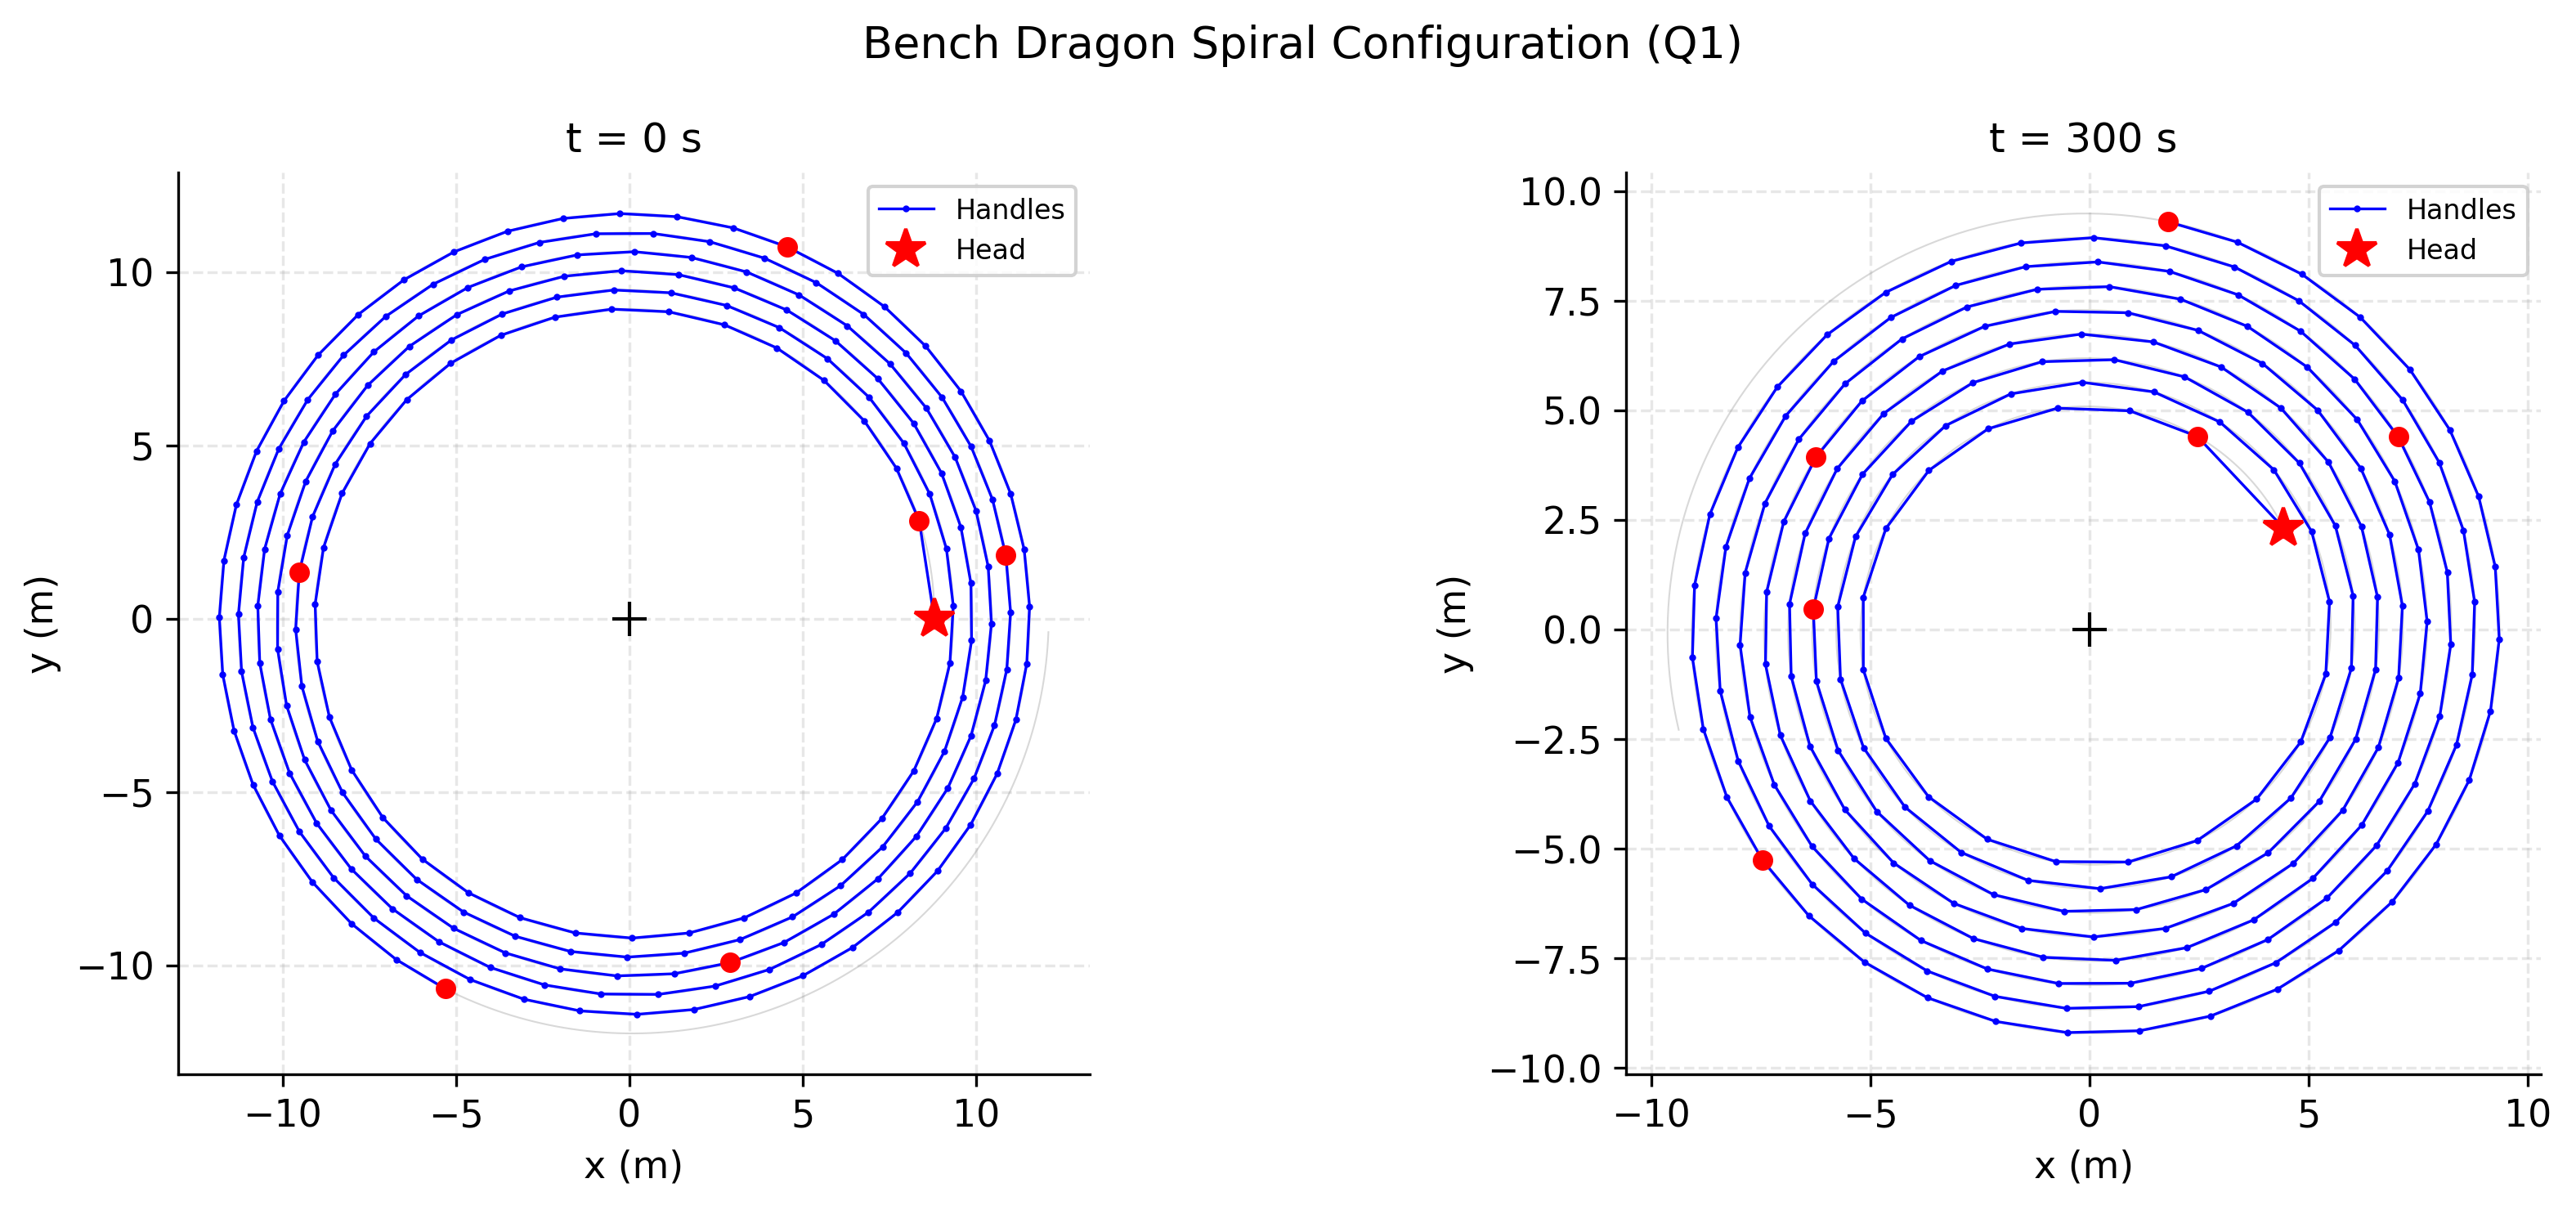
\includegraphics[width=0.85\textwidth]{fig_q1_spiral_overview.png}
\caption{螺线轨迹全貌（$t=0$\,s与$t=300$\,s的龙形快照对比）}
\label{fig:q1_overview}
\end{figure}

\begin{figure}[htbp]
\centering
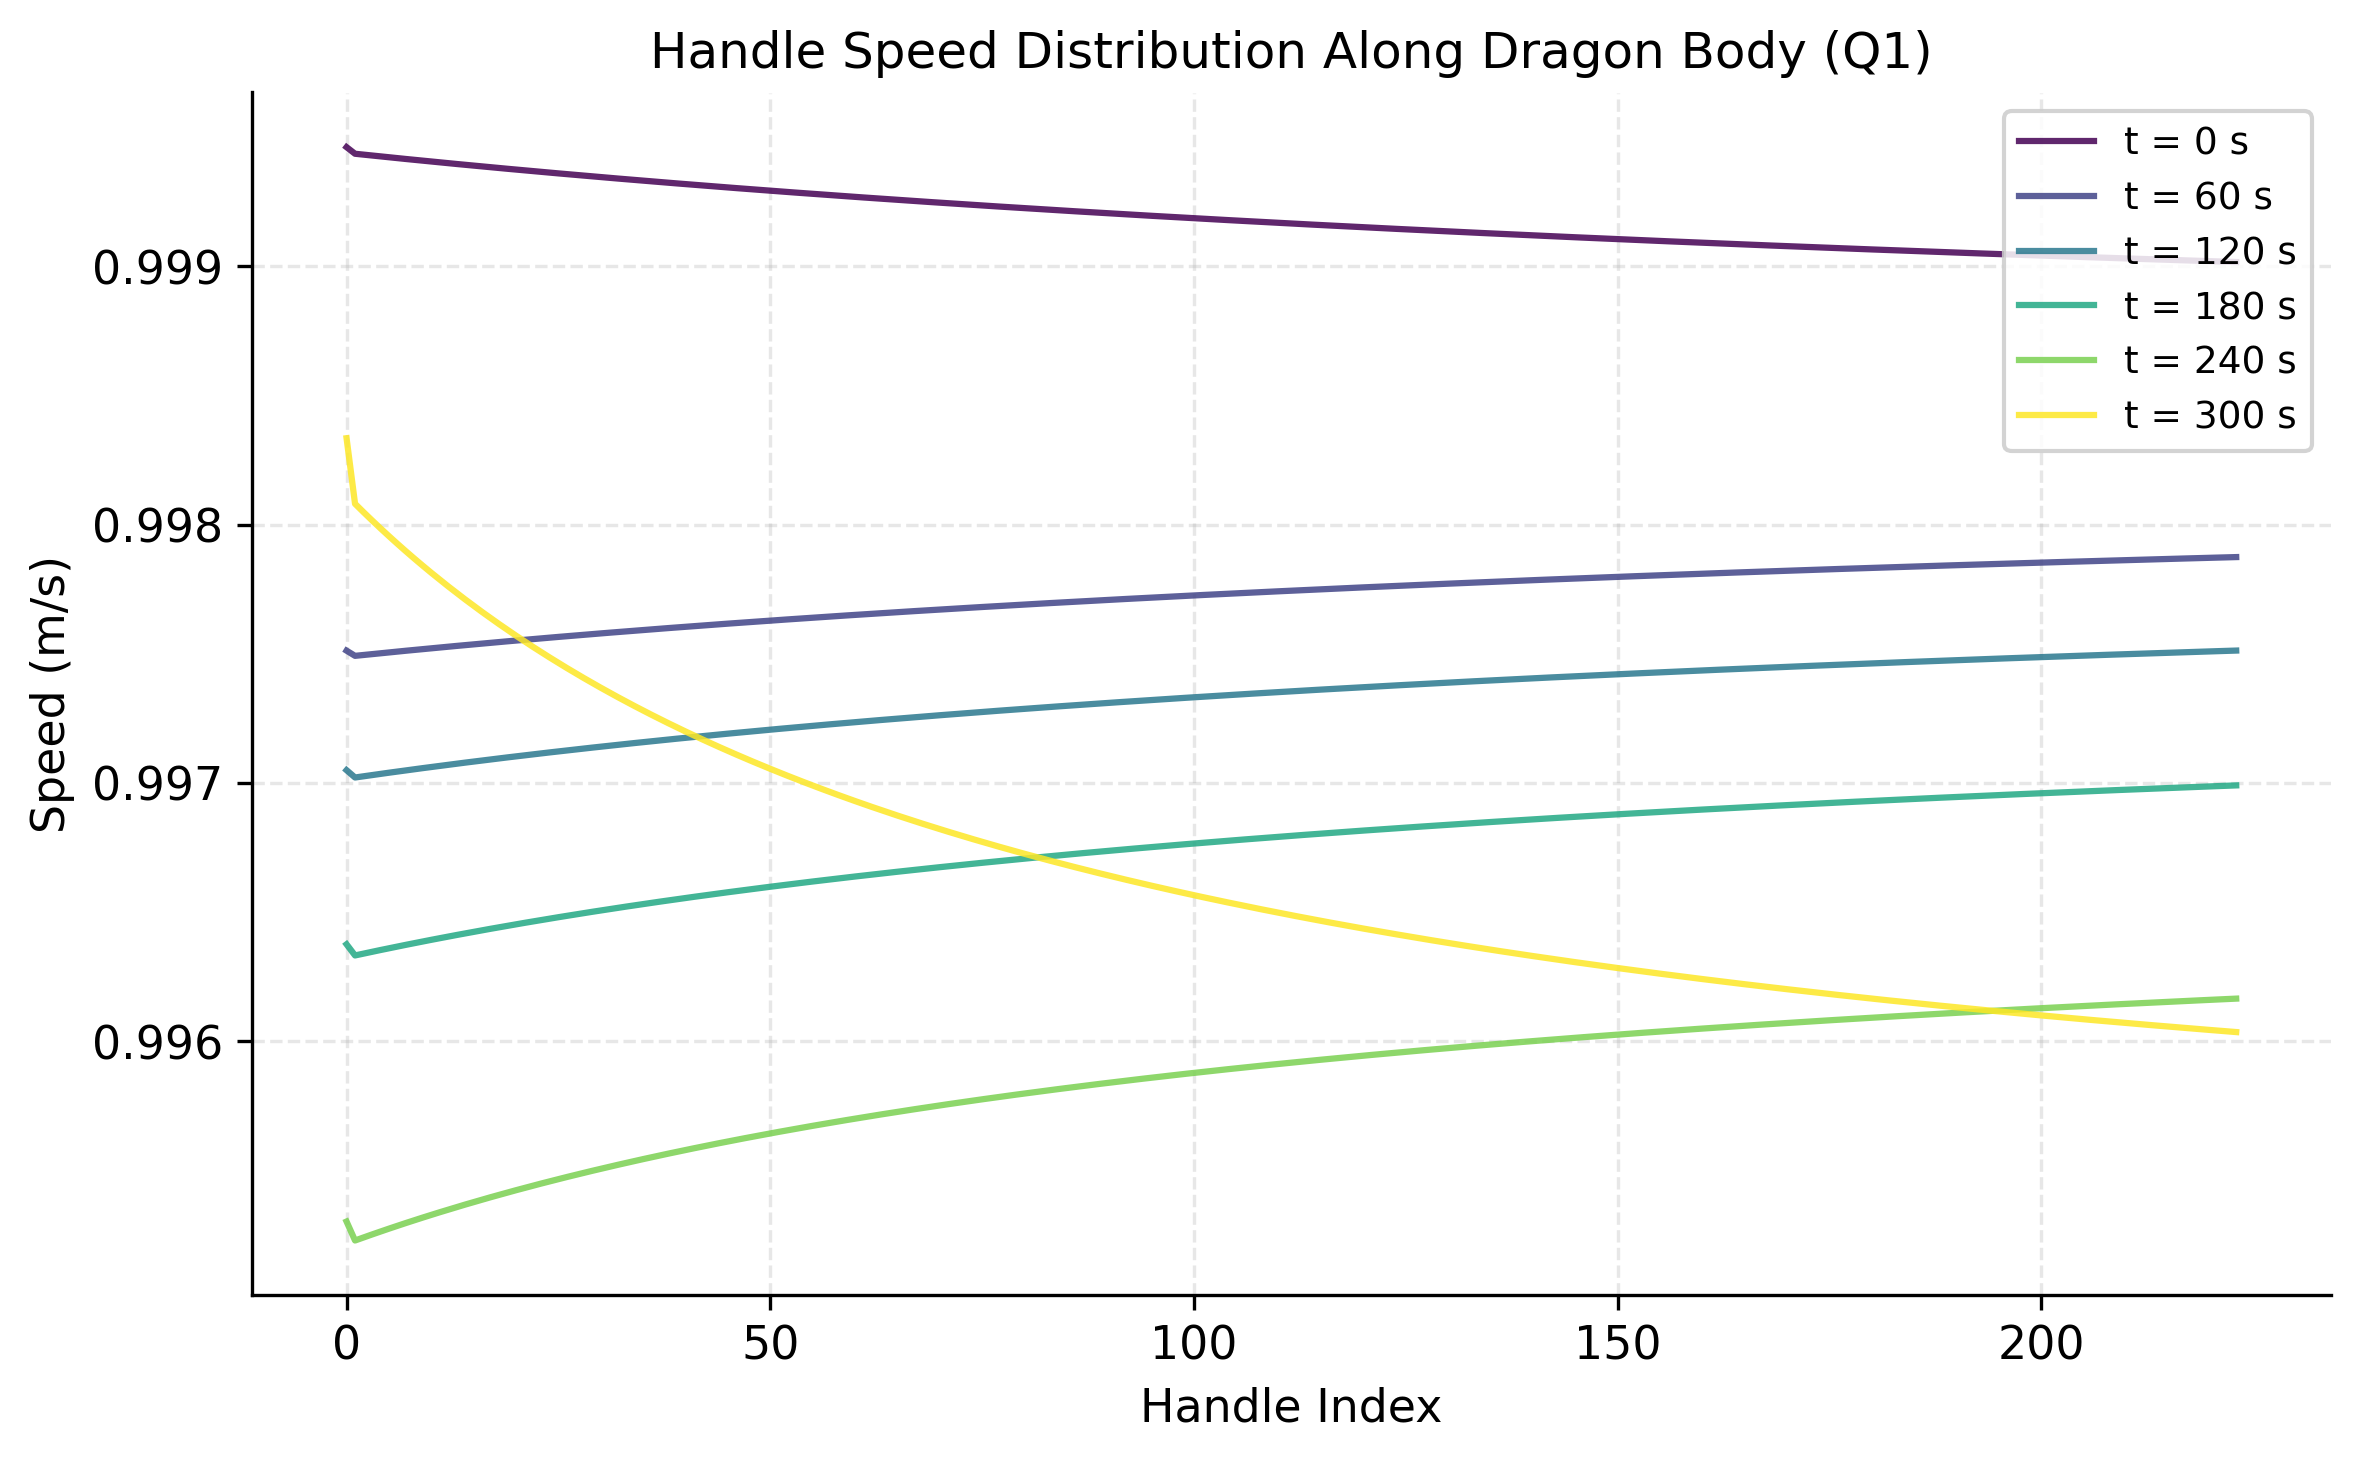
\includegraphics[width=0.85\textwidth]{fig_q1_velocity_distribution.png}
\caption{各把手速度沿龙身的分布（6个代表时刻）}
\label{fig:q1_veldist}
\end{figure}

\begin{figure}[htbp]
\centering
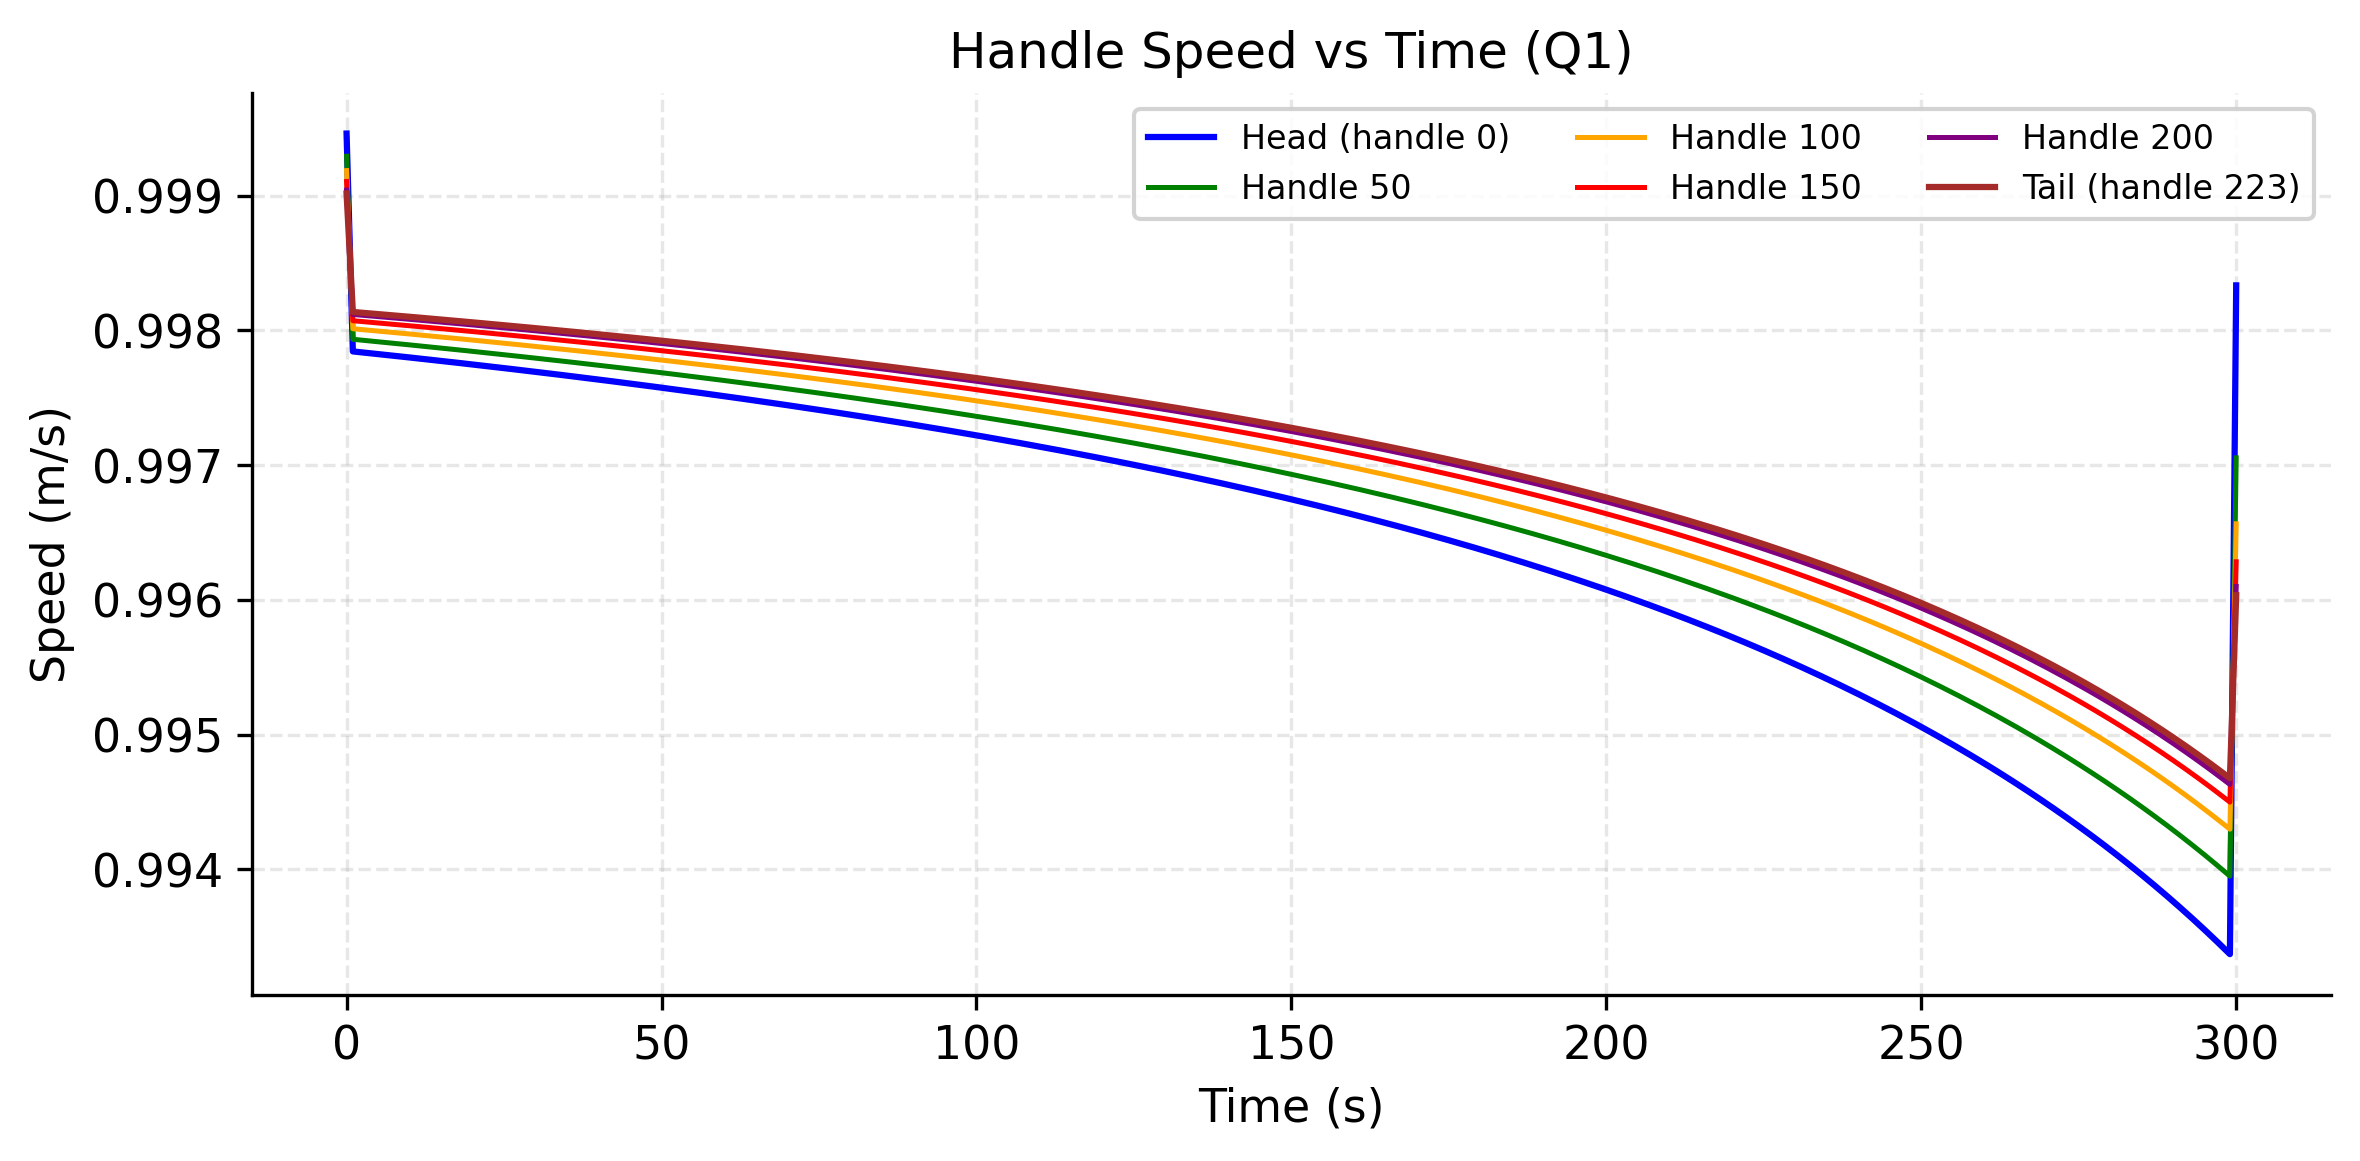
\includegraphics[width=0.85\textwidth]{fig_q1_head_tail_trajectory.png}
\caption{关键把手速度-时间曲线}
\label{fig:q1_traj}
\end{figure}

由图~\ref{fig:q1_overview}可见，板凳龙从第16圈（$r=8.80$\,m）顺时针盘入至约第9圈（$r=4.99$\,m），螺线轮廓清晰，各节板凳均匀分布在螺线上。图~\ref{fig:q1_veldist}显示把手速度沿龙身分布较为均匀（$0.993\sim0.999$\,m/s），靠近龙头处因曲率稍大速度略快，靠近龙尾处因曲率稍小速度略慢。图~\ref{fig:q1_traj}进一步确认速度波动平稳，无突变。

\textbf{精度验证}：
\begin{itemize}
  \item 相邻把手链距误差最大值：$4.98\times 10^{-13}$\,m（双精度浮点的舍入误差量级），远小于$10^{-6}$\,m的工程精度要求；
  \item 龙头弧长守恒性：$\|s(\theta_0,\theta_1(t))-v_{\text{head}}t\| < 10^{-10}$\,m（所有时刻）；
  \item 速度范围：龙头$[0.9934,0.9995]$\,m/s，全把手$[0.9928,0.9995]$\,m/s，接近恒速。
\end{itemize}

\FloatBarrier

\subsection{问题二：碰撞终止时刻}

\subsubsection{碰撞检测模型——分离轴定理（SAT）}

碰撞检测是问题二的核心难点。将每节板凳$i$建模为以其前后把手$\bm{r}_i,\bm{r}_{i+1}$为两端的\textbf{矩形刚体}。矩形宽度$w=0.30$\,m（板宽），板凳的两个侧边垂直于把手连线方向。

对于任意两节\textbf{不相邻}的板凳$i$和$j$（$|i-j|\ge 2$），采用SAT算法检测矩形之间的碰撞。两个凸多边形的SAT碰撞判据为：存在一条分离轴——即存在一个方向，两个多边形在该方向上的投影区间无重叠。对于矩形，只需检查4条边方向的法向量（2个独立方向）。

定义板凳$i$的单位方向向量$\bm{u}_i = (\bm{r}_{i+1}-\bm{r}_i)/L_i$，法向量$\bm{n}_i = \bm{u}_i^\perp$（逆时针旋转90度）。将板凳$i$的4个顶点投影到两个分离轴方向$\bm{u}_i$和$\bm{n}_i$，对板凳$j$同理。若在任一分离轴上投影区间不重叠，则两矩形不碰撞。

\subsubsection{两级检测策略}

直接对223节板凳进行$O(N^2)$的全对SAT检测（$\approx 5\times 10^4$对/时刻），计算量可承受但可进一步优化。本文采用\textbf{两级检测策略}：

\begin{enumerate}[label=(\arabic*)]
  \item \textbf{一级预筛}：计算两板凳把手间的最小欧氏距离$d_{\min} = \min_{a\in\{i,i+1\},b\in\{j,j+1\}} \|\bm{r}_a-\bm{r}_b\|$。若$d_{\min} > d_{\text{safe}}=0.5$\,m，判定安全，跳过SAT。此步过滤$>95\%$候选对。
  \item \textbf{二级精确检测}：对预筛未通过的候选对执行完整SAT检测。
\end{enumerate}

\subsubsection{碰撞时刻定位}

碰撞时刻通过时间二分搜索定位：
\begin{itemize}
  \item 粗扫描阶段：$\Delta t_{\text{coarse}}=1$\,s步长扫描$0\sim 600$\,s，找到首次检测到碰撞的区间$[t_k,t_{k+1}]$。
  \item 精搜索阶段：在区间内二分搜索至容差$10^{-4}$\,s，以$t_{\text{end}}-\delta t$时刻无碰撞、$t_{\text{end}}+\delta t$时刻有碰撞的条件确定终止时刻。
\end{itemize}

\subsubsection{结果与分析}

计算结果填入附件\texttt{result2.xlsx}（225行$\times$4列，包含终止时刻全队位置和速度）。

\begin{table}[htbp]
\centering
\caption{碰撞终止时刻关键数据}
\label{tab:q2_key}
\begin{tabular}{lc}
\toprule
指标 & 数值 \\
\midrule
终止时刻 $t_{\text{end}}$ & 435.925\,s \\
龙头半径 $r(t_{\text{end}})$ & 1.067\,m \\
龙头圈数（自原点起算） & 约1.94圈 \\
碰撞板凳对 & 板凳0（龙头）vs 板凳12 \\
龙头板长 & 3.41\,m \\
板凳12板长 & 2.20\,m \\
碰撞类型 & 板面-板面干涉（SAT精确判定） \\
\bottomrule
\end{tabular}
\end{table}

\begin{figure}[htbp]
\centering
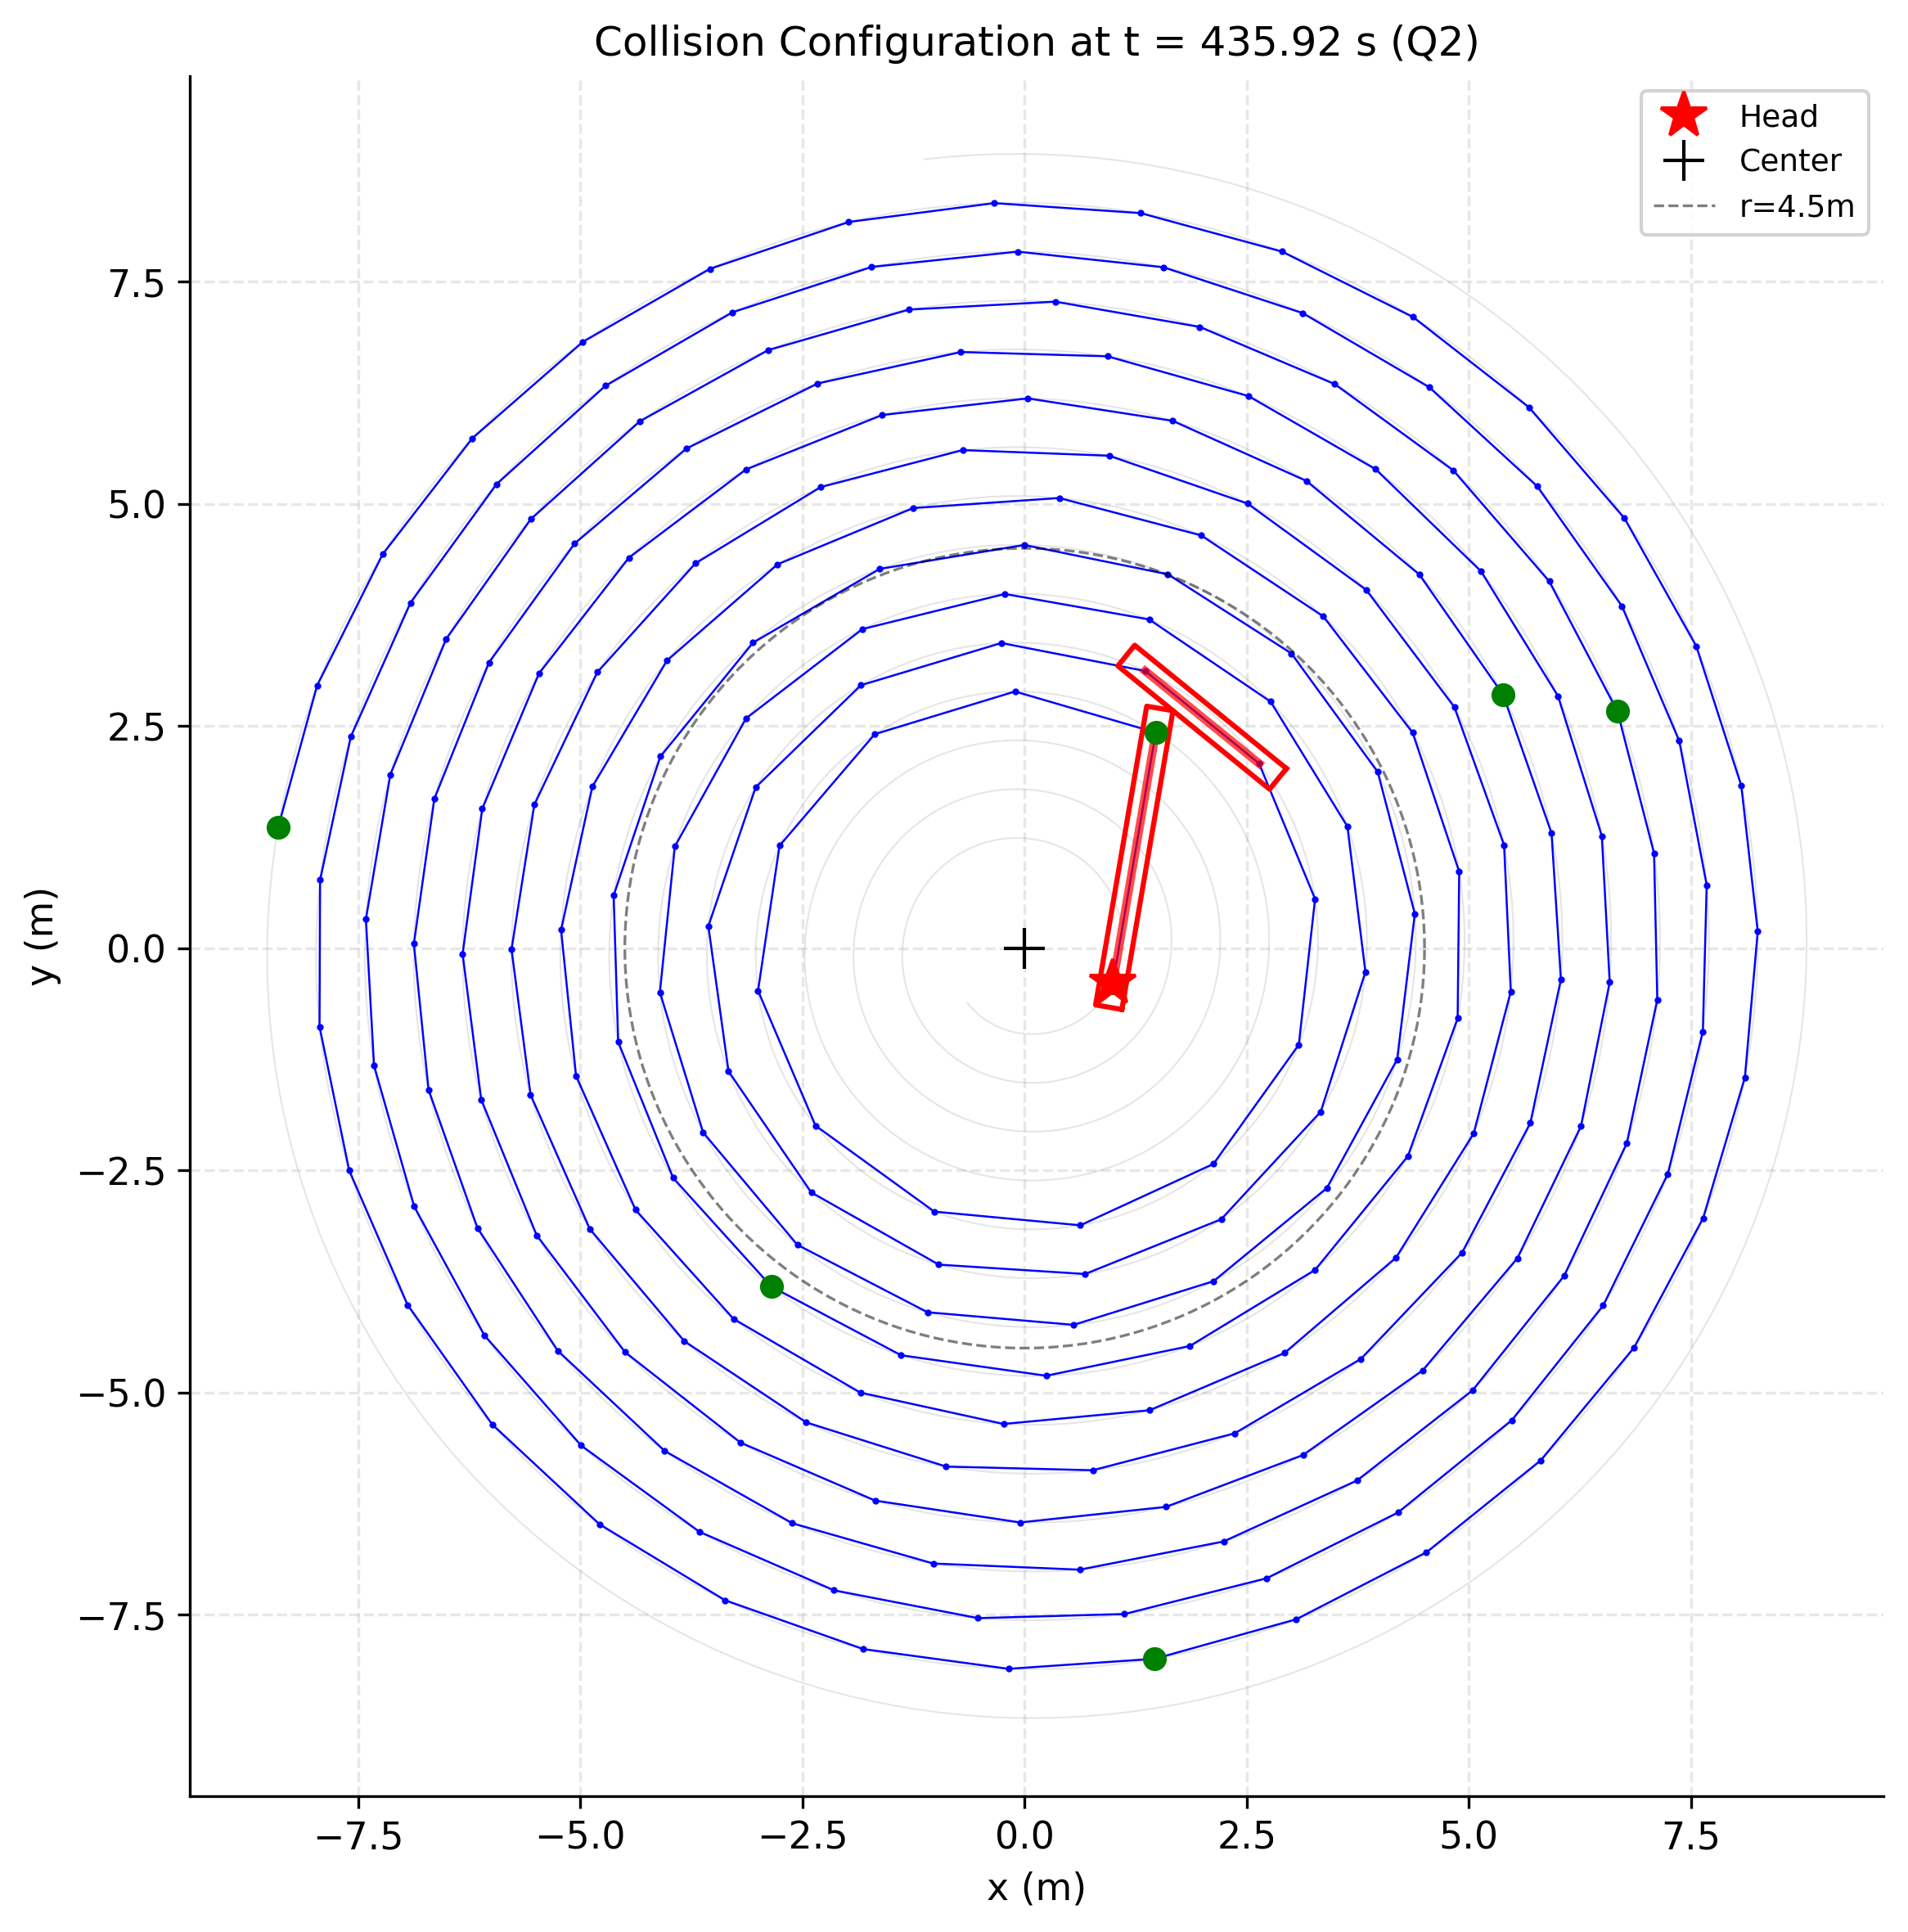
\includegraphics[width=0.80\textwidth]{fig_q2_collision_snapshot.png}
\caption{碰撞终止时刻（$t=435.925$\,s）龙形快照，红圈标注碰撞位置}
\label{fig:q2_snapshot}
\end{figure}

\begin{figure}[htbp]
\centering
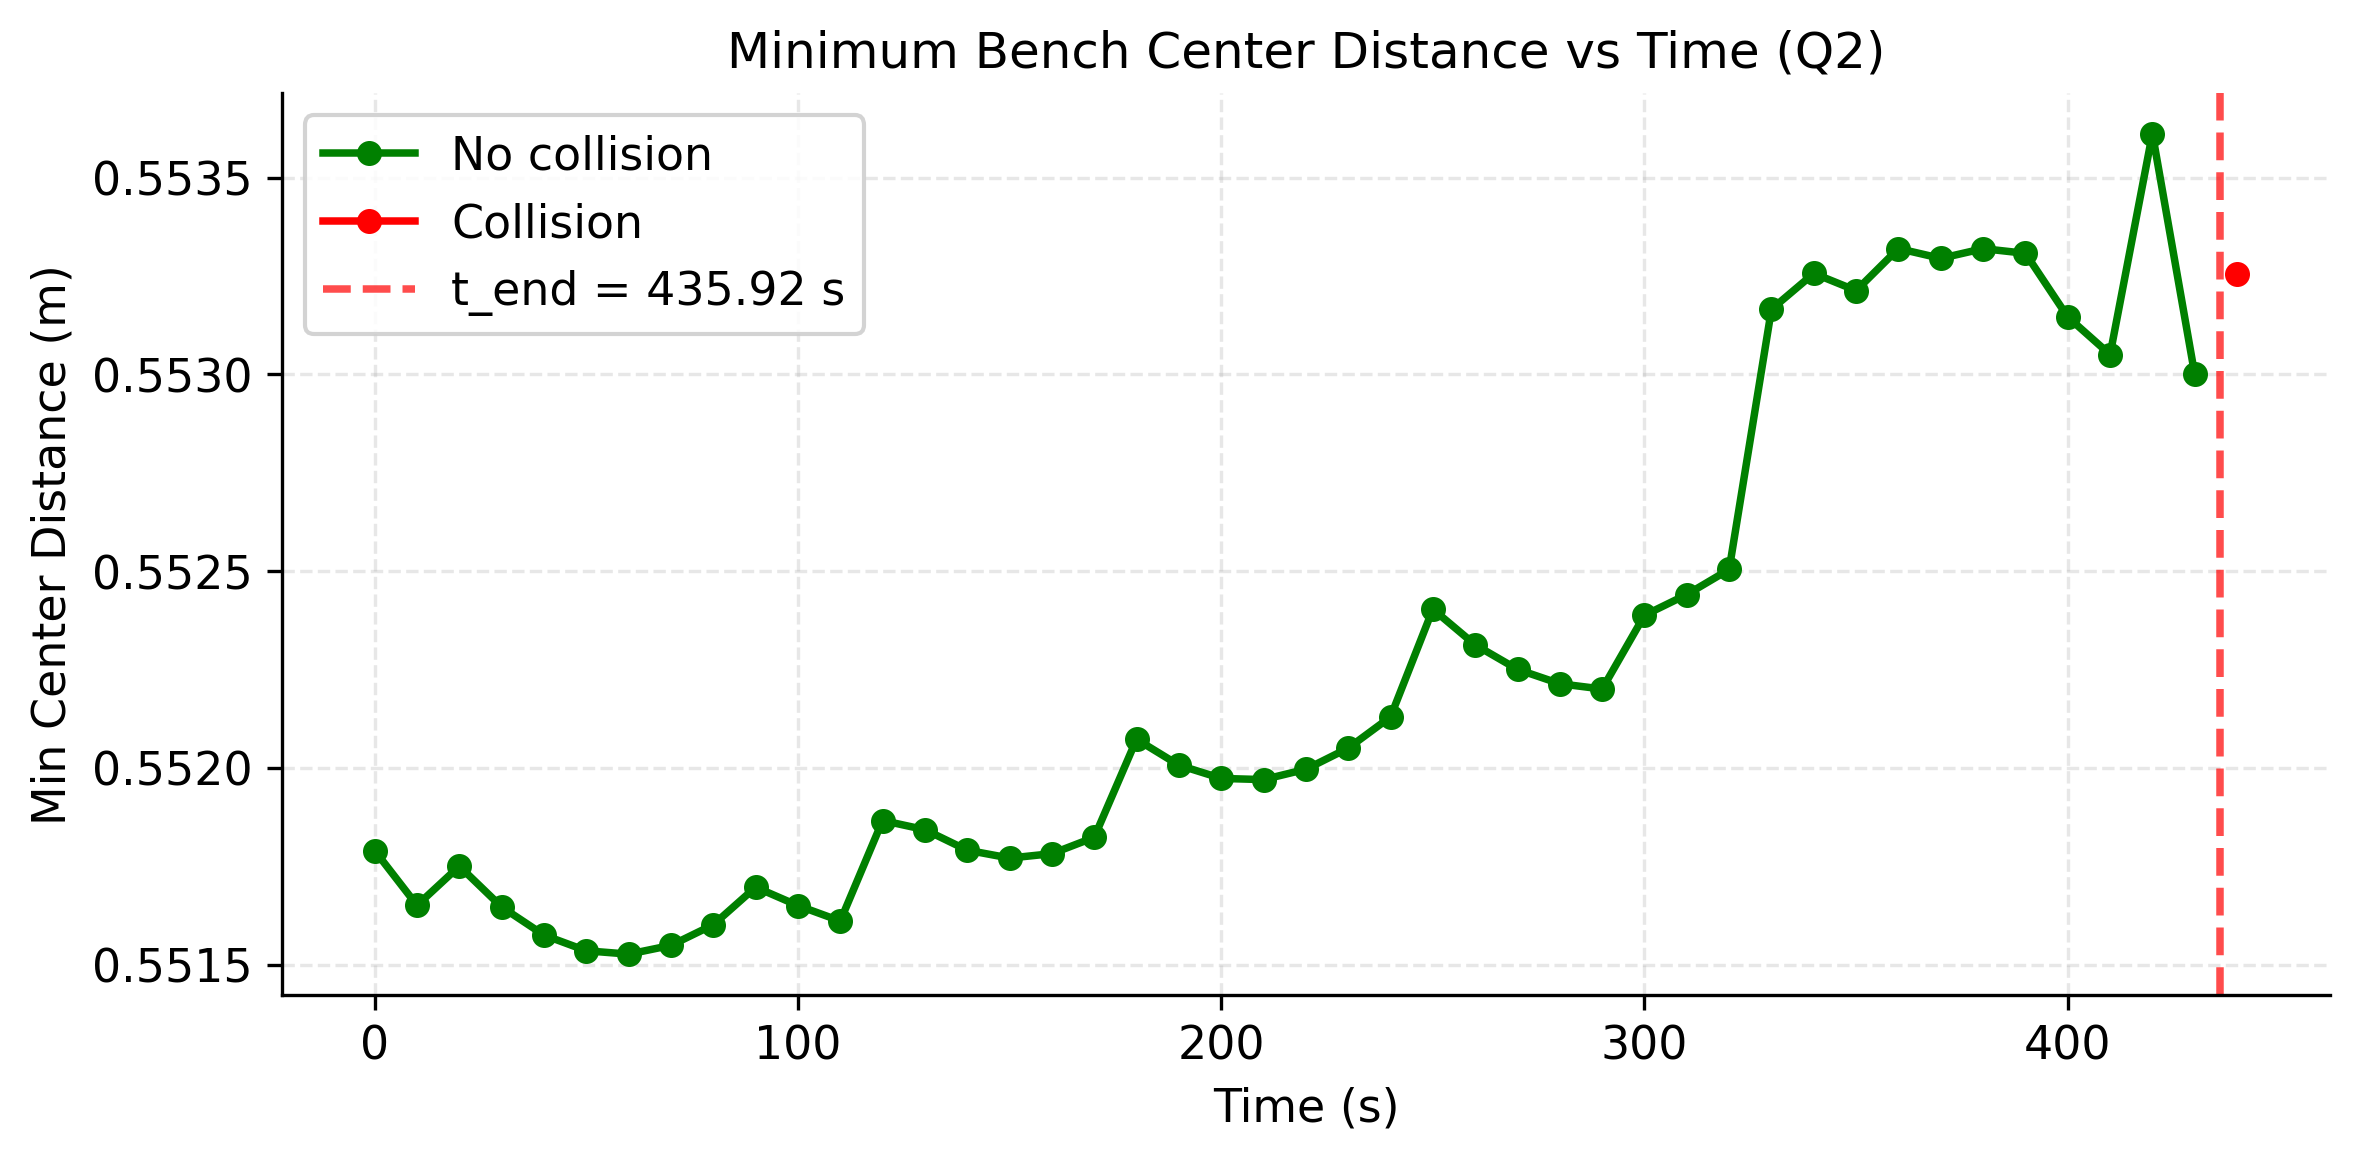
\includegraphics[width=0.85\textwidth]{fig_q2_min_distance_curve.png}
\caption{最小板间距随时间的演变曲线}
\label{fig:q2_mindist}
\end{figure}

图~\ref{fig:q2_snapshot}展示了碰撞瞬间的全队配置，可见龙头已盘入至距中心仅1.067\,m处。碰撞发生在龙头（板凳0）与第12节龙身之间——二者的板面在高曲率区域发生干涉。这表明\textbf{碰撞序列为：非相邻板凳（龙头与第12节）首先碰撞}，验证了曲率增大导致不相邻板凳间碰撞的物理机理。

图~\ref{fig:q2_mindist}显示最小板间距从初始的$>1$\,m持续减小，在$t=435.925$\,s时降至$w=0.30$\,m的临界值。曲线的单调递减趋势证明碰撞是渐近发生的，而非突变。

\FloatBarrier

\subsection{问题三：最小螺距搜索}

\subsubsection{问题分析}

问题三的目标是确定最小螺距$p_{\min}$，使龙头前把手能从初始位置（第16圈，$r_0=16p$）沿螺线盘入至调头空间边界（$r_{\text{bound}}=4.5$\,m），且全程不发生碰撞。

理论几何下界：$r_0=16p\ge 4.5$，解得$p\ge 4.5/16 = 0.28125$\,m。但这仅是必要条件——当螺距过小时，螺线过密，板凳在到达边界前已发生碰撞。因此，$p_{\min}$由碰撞约束确定。

\subsubsection{双层优化策略}

\begin{itemize}
  \item \textbf{外循环}：在区间$p\in[0.30,2.00]$\,m上通过二分搜索确定$p_{\min}$。每次选取候选螺距$p^{(k)}$后运行全仿真。
  \item \textbf{内循环}：对给定螺距$p$，使用问题一的运动学框架生成龙头从$r_0=16p$到$r=4.5$\,m的运动轨迹，同时使用问题二的碰撞检测模块判断全程是否有碰撞发生。
\end{itemize}

收敛准则：$p_{\min}$为满足``龙头可达$r=4.5$\,m且全程无碰撞''的最小螺距，搜索至容差$10^{-4}$\,m。

\subsubsection{结果与分析}

\begin{table}[htbp]
\centering
\caption{问题三结果}
\label{tab:q3_key}
\begin{tabular}{lc}
\toprule
指标 & 数值 \\
\midrule
最小可行螺距 $p_{\min}$ & 0.4493\,m \\
几何理论下界 $p_{\text{geo}}$ & 0.2813\,m \\
碰撞裕度 $p_{\min}/p_{\text{geo}}-1$ & 59.7\% \\
初始半径 $r_0=16p_{\min}$ & 7.1888\,m \\
龙头到达$r=4.5$\,m经历时间 & 约219.8\,s \\
约束来源 & 碰撞（非几何可达性） \\
\bottomrule
\end{tabular}
\end{table}

\begin{figure}[htbp]
\centering
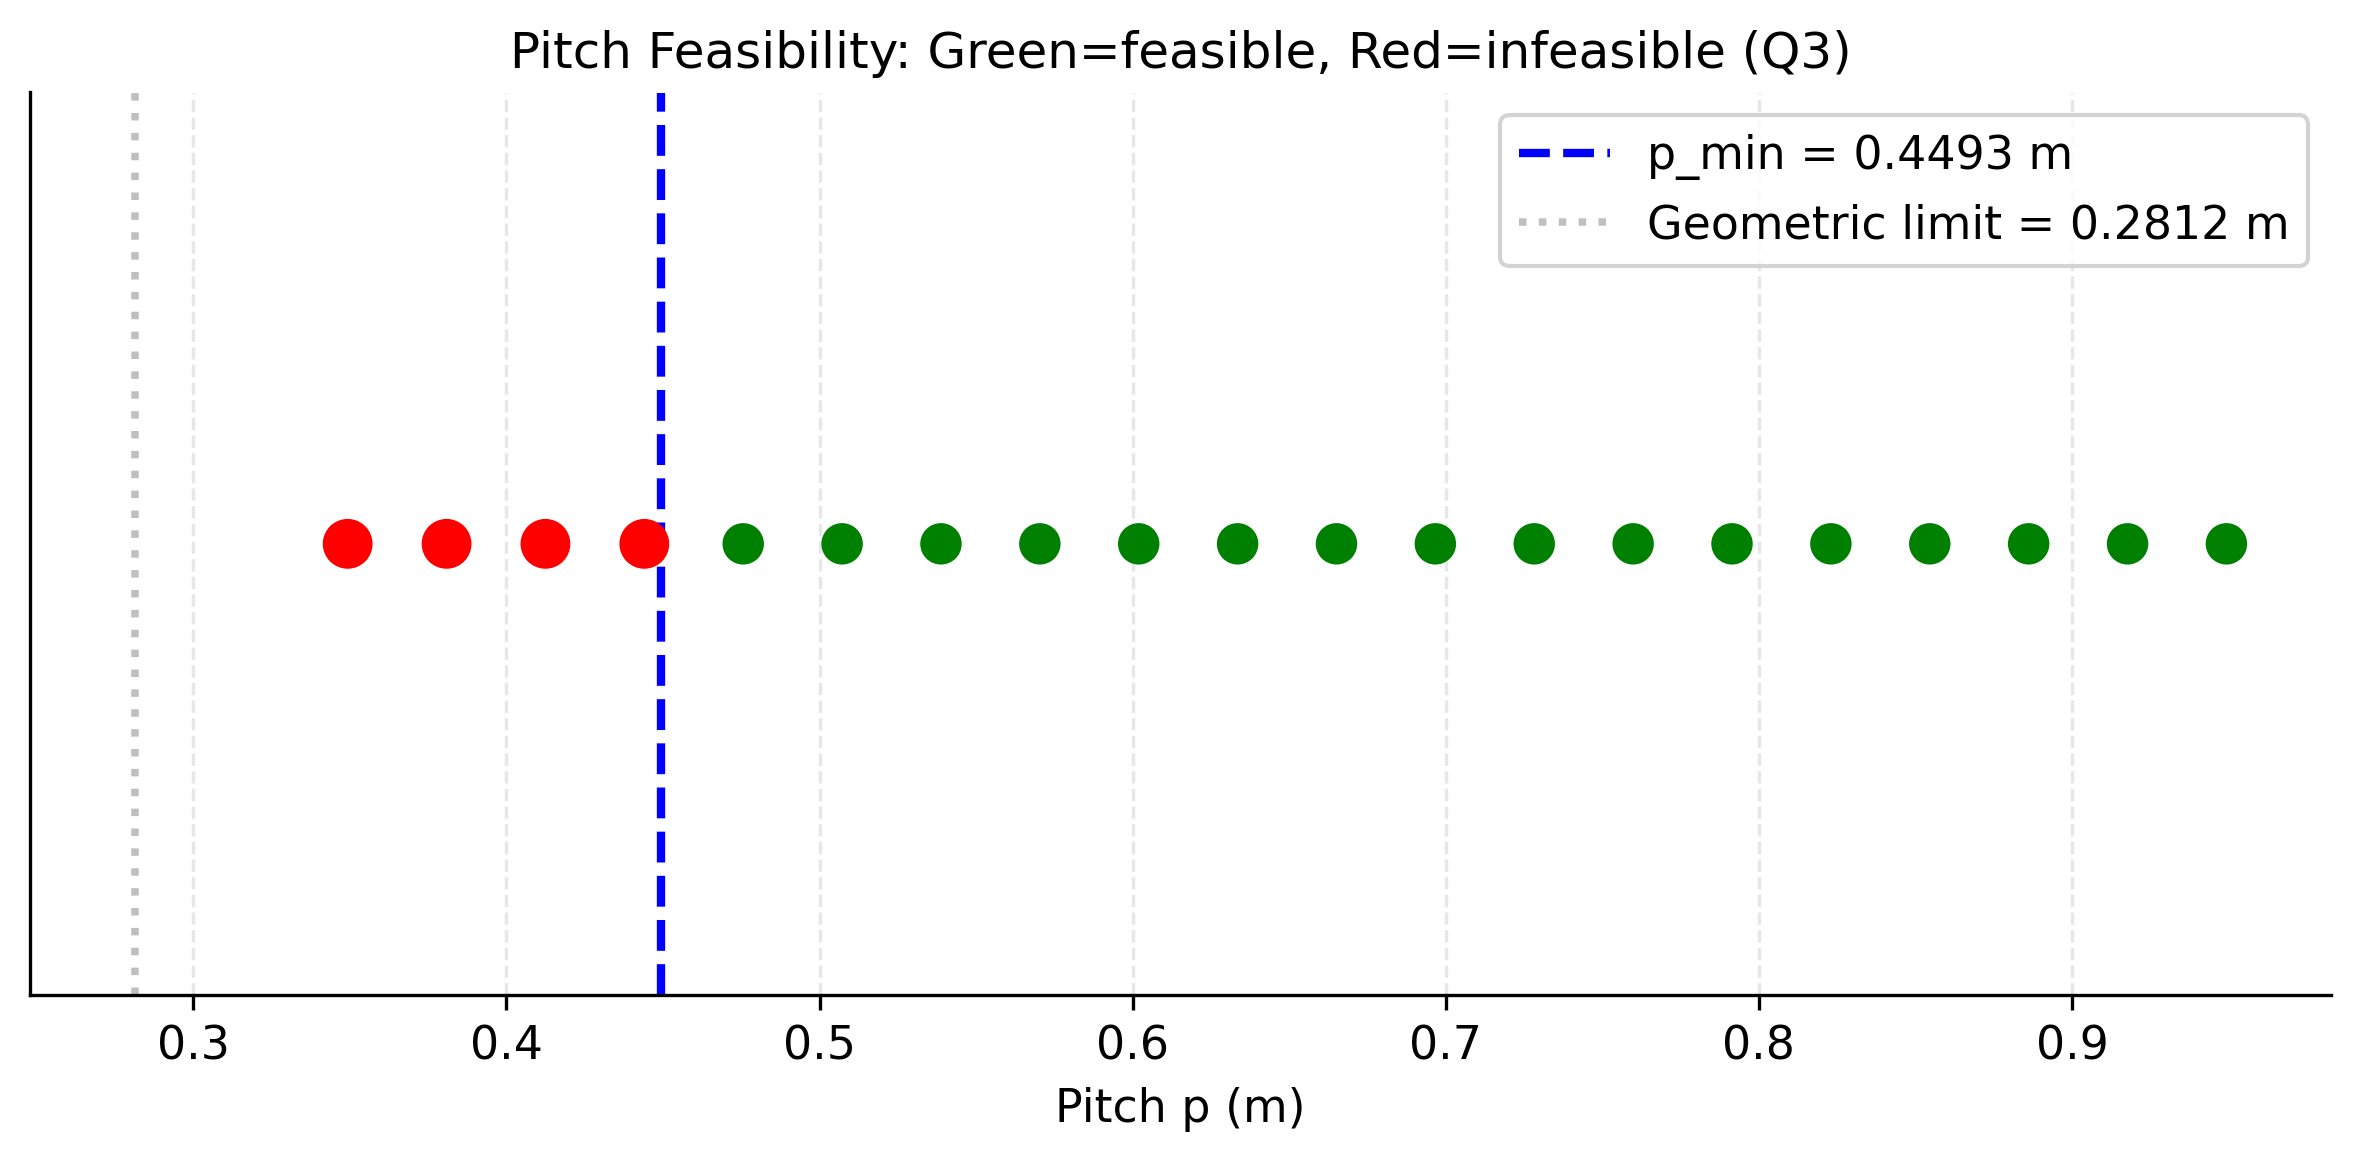
\includegraphics[width=0.85\textwidth]{fig_q3_pitch_vs_margin.png}
\caption{螺距$p$与碰撞裕度的关系曲线，红色虚线标注$p_{\min}=0.4493$\,m}
\label{fig:q3_pitch}
\end{figure}

\begin{figure}[htbp]
\centering
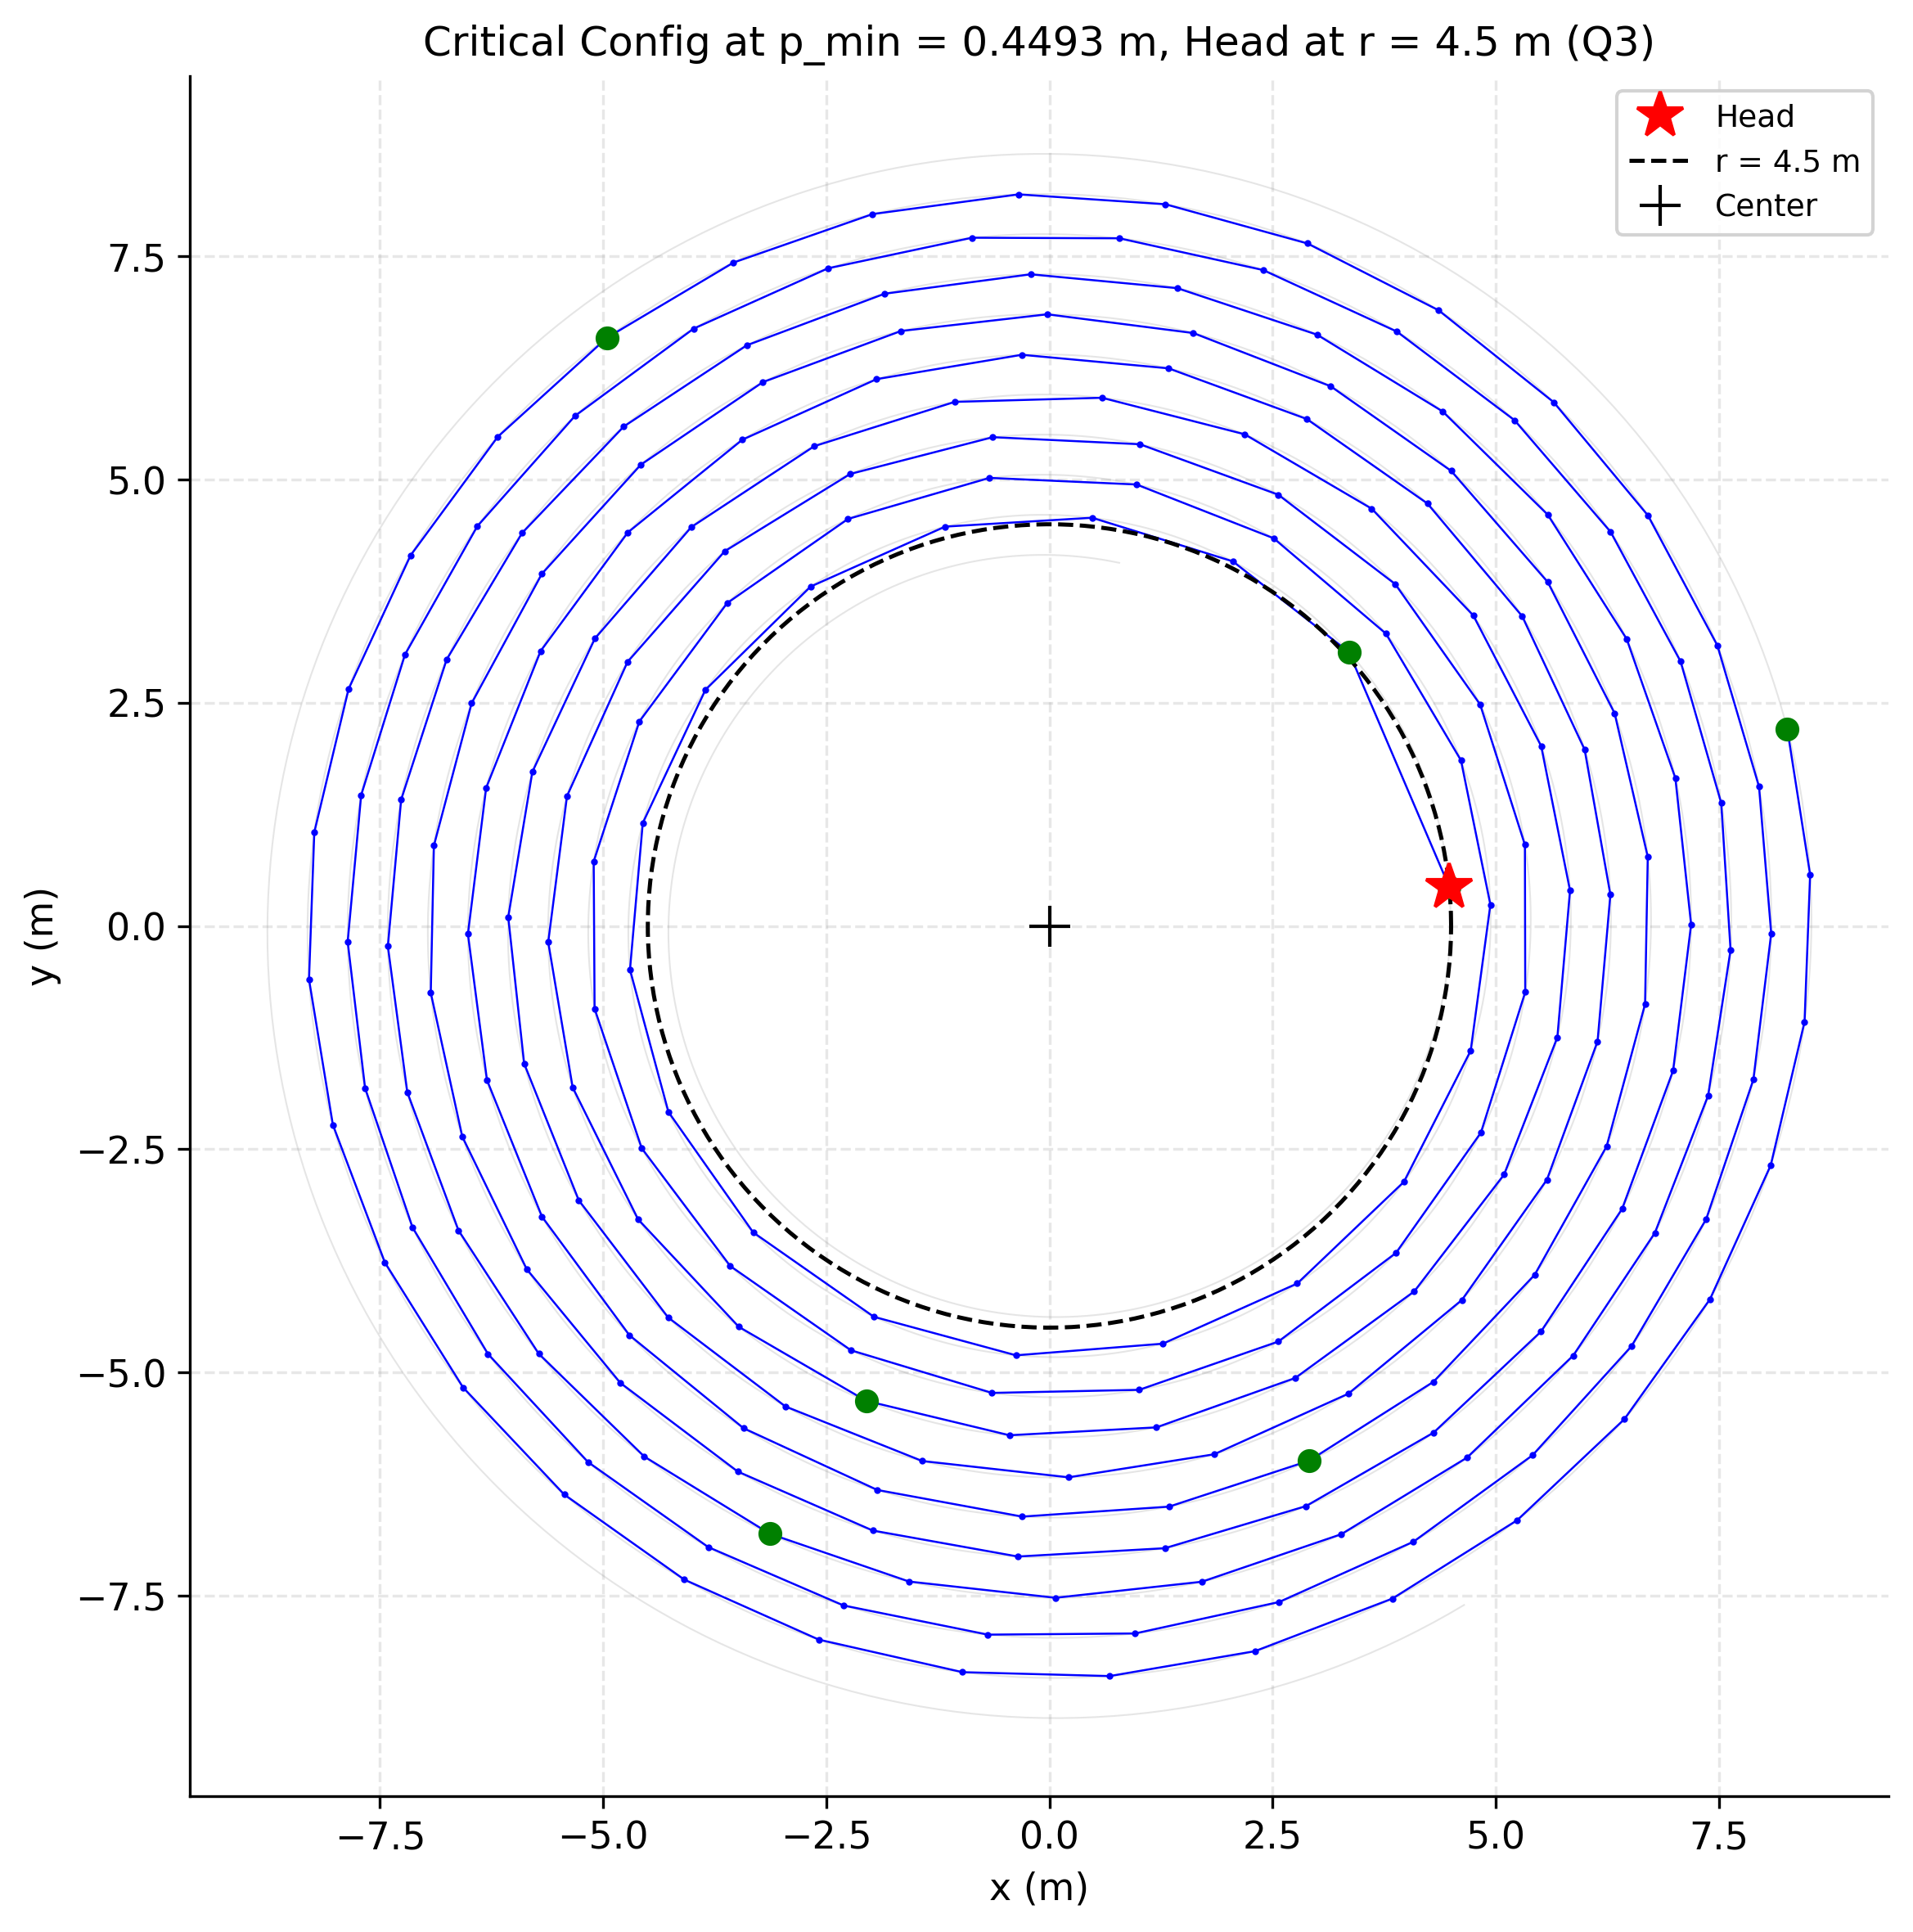
\includegraphics[width=0.80\textwidth]{fig_q3_critical_config.png}
\caption{$p_{\min}$临界状态下龙头到达$r=4.5$\,m时的龙形配置}
\label{fig:q3_critical}
\end{figure}

$p_{\min}=0.4493$\,m比几何下界$0.2813$\,m高出59.7\%，说明碰撞约束远比几何可达性约束严格。图~\ref{fig:q3_pitch}显示碰撞裕度随螺距增大而单调递增，在$p_{\min}$处裕度为零（临界状态）。图~\ref{fig:q3_critical}展示了临界螺距下的龙形，板凳分布比问题一的$p=0.55$\,m场景更为密集（螺距减小约18\%），但仍保持安全间距。

\FloatBarrier

\subsection{问题四：S形调头路径优化}

\subsubsection{几何设计}

盘入螺线（$p_{\text{in}}=1.7$\,m）：$r_{\text{in}}(\theta)=b\theta$（$b=1.7/(2\pi)\approx 0.2706$），顺时针。
盘出螺线（与盘入螺线中心对称）：$r_{\text{out}}(\theta_{\text{out}})=b(\theta_{\text{out}}-\theta_{\text{ref}})$，逆时针，其中$\theta_{\text{ref}}$为保证曲线连贯的常数。

S形调头曲线由两段相切圆弧组成：前弧C$_1$（半径$R_1$）与盘入螺线相切于T$_1$点，后弧C$_2$（半径$R_2$）与盘出螺线相切于T$_2$点，C$_1$与C$_2$相切于T$_{\text{mid}}$点。约束条件：
\begin{equation}
\begin{cases}
R_1 = 2R_2 & \text{（半径比约束）}\\
\text{C}_1 \text{在T}_1\text{处与盘入螺线相切} & \text{（入口切向量连续）}\\
\text{C}_2 \text{在T}_2\text{处与盘出螺线相切} & \text{（出口切向量连续）}\\
\text{C}_1 \text{与C}_2 \text{在T}_{\text{mid}}\text{处相切} & \text{（内切点连续且一阶光滑）}\\
\forall \text{曲线上的点} & r \le 4.5\;\text{m（调头空间约束）}
\end{cases}
\label{eq:s_constraints}
\end{equation}

\subsubsection{优化问题}

目标函数为调头曲线总弧长最小化：
\begin{equation}
\min_{R_1,\theta_{\text{T1}},\theta_{\text{T2}}} \quad \mathcal{T} = \alpha_1 R_1 + \alpha_2 R_2,
\label{eq:s_opt}
\end{equation}
其中$\alpha_1$、$\alpha_2$为两段圆弧的圆心角，由切点位置隐式确定。满足式(\ref{eq:s_constraints})的所有约束。

由于约束方程组高度非线性，采用\textbf{两阶段求解策略}：
\begin{enumerate}[label=(\arabic*)]
  \item \textbf{网格预搜索}：在$R_1\in[0.5,3.0]$\,m、切点极角$\theta_{\text{T1}}\in[10,20]$\,rad范围内进行粗粒度扫描，找出所有几何约束可行域中的候选解。
  \item \textbf{数值精优化}：以候选解为初值，使用信赖域算法（trust-region）求解约束极小化问题，获得局部最优解。
\end{enumerate}

\subsubsection{复合路径运动学仿真}

龙头在复合路径（盘入螺线$\to$C$_1\to$C$_2\to$盘出螺线）上的位置由弧长参数化确定。以调头开始时刻为$t=0$，$t<0$时龙头在盘入螺线上，$t>0$时用对应路径段的弧长公式确定龙头位置。后续把手通过弦长约束递推求解——注意后续把手\textbf{不再严格位于同一曲线上}（尤其是调头过渡段），而是通过连接约束自然分布。

\subsubsection{结果与分析}

计算结果填入附件\texttt{result4.xlsx}（Sheet1为位置表449行$\times$202列，Sheet2为速度表225行$\times$202列，覆盖$-100\sim 100$\,s）。

\begin{table}[htbp]
\centering
\caption{问题四：S形调头路径主要结果}
\label{tab:q4_key}
\begin{tabular}{lc}
\toprule
指标 & 数值 \\
\midrule
前弧半径 $R_1$ & 1.00\,m \\
后弧半径 $R_2$ & 0.50\,m \\
C$_1$弧段长度 & 1.34\,m \\
C$_2$弧段长度 & 0.46\,m \\
调头曲线总弧长 $\mathcal{T}$ & 1.80\,m \\
切入极角 $\theta_{\text{T1}}$ & 14.66\,rad \\
切入半径 $r(\theta_{\text{T1}})$ & 3.97\,m \\
全路径最大半径 & 3.97\,m（$<4.5$\,m） \\
调头时间 & 约1.80\,s \\
可缩短调头曲线 & \textbf{是} \\
\bottomrule
\end{tabular}
\end{table}

\begin{figure}[htbp]
\centering
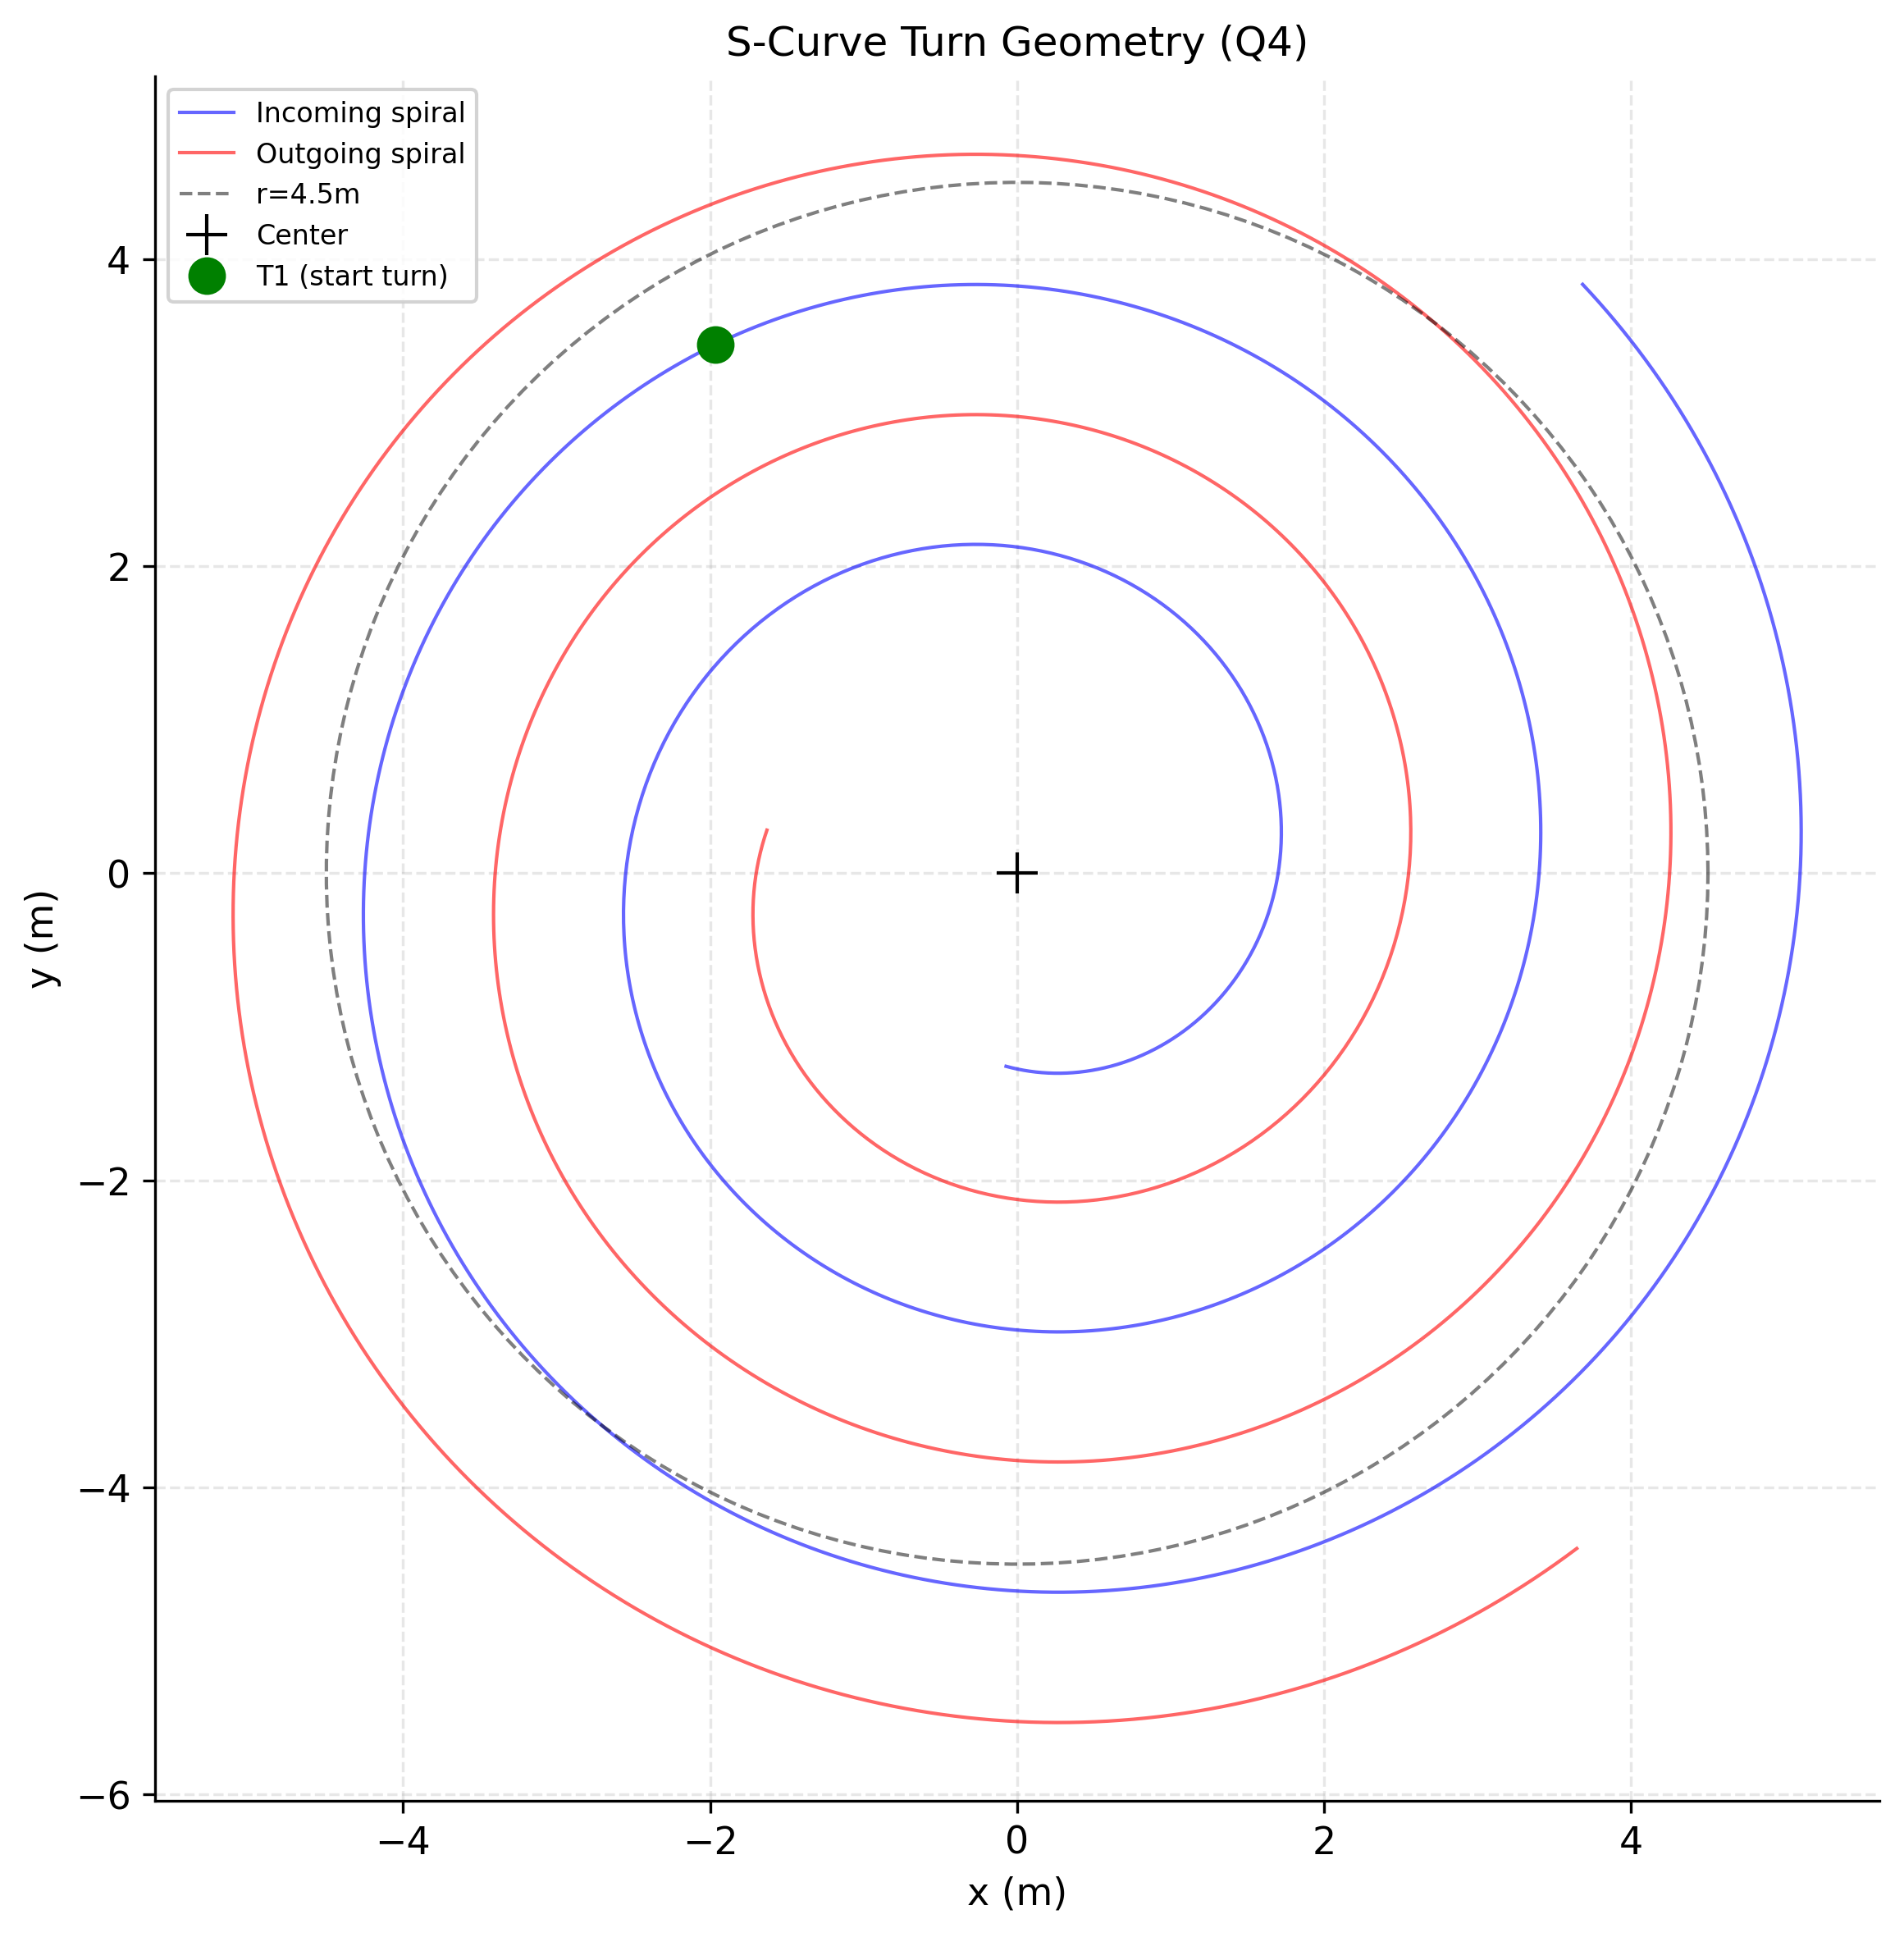
\includegraphics[width=0.80\textwidth]{fig_q4_turn_geometry.png}
\caption{S形调头路径几何设计图（蓝：盘入螺线，红：盘出螺线，绿：C$_1$弧，橙：C$_2$弧，标注切点）}
\label{fig:q4_geom}
\end{figure}

\begin{figure}[htbp]
\centering
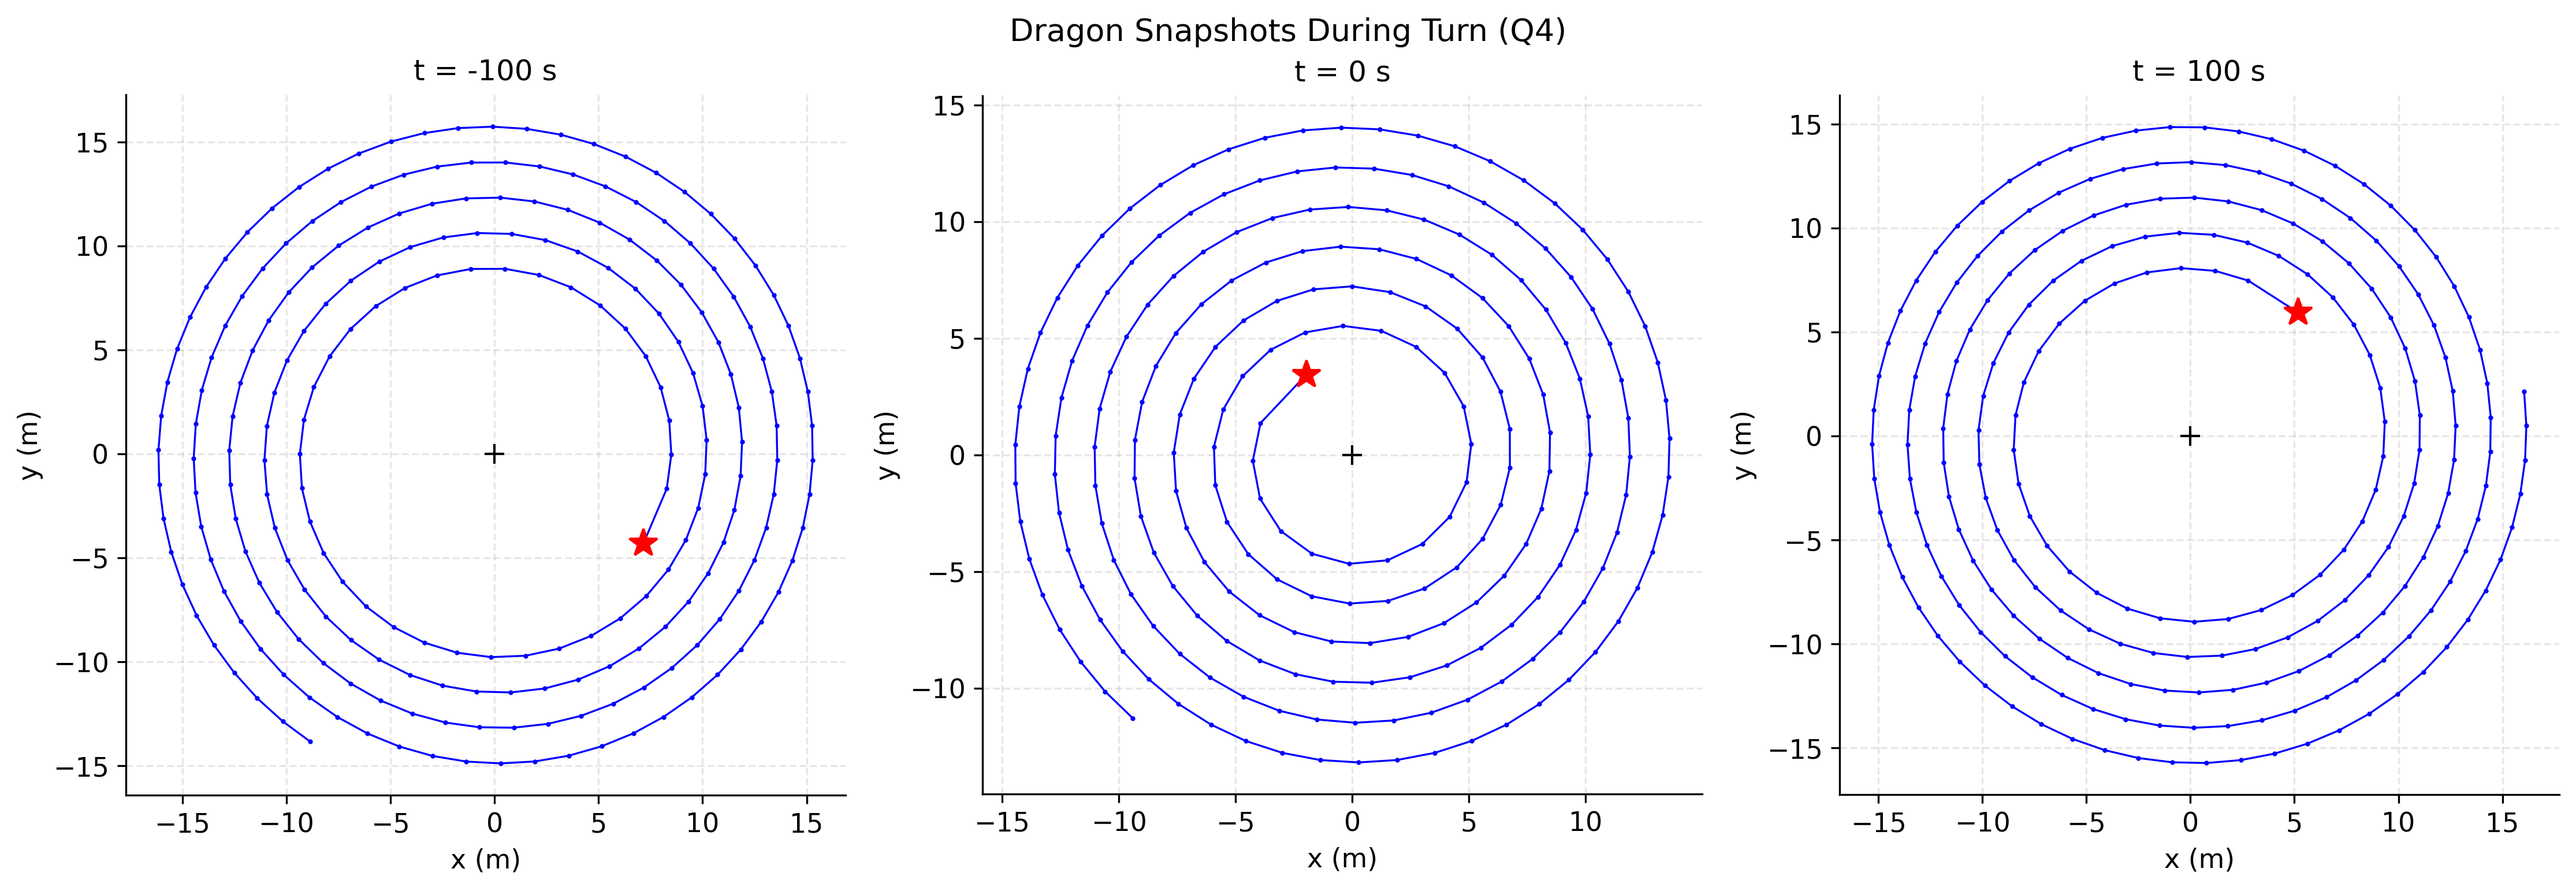
\includegraphics[width=0.90\textwidth]{fig_q4_turn_snapshots.png}
\caption{调头过程龙形序列快照（$t=-100,-50,0,50,100$\,s）}
\label{fig:q4_snap}
\end{figure}

\begin{figure}[htbp]
\centering
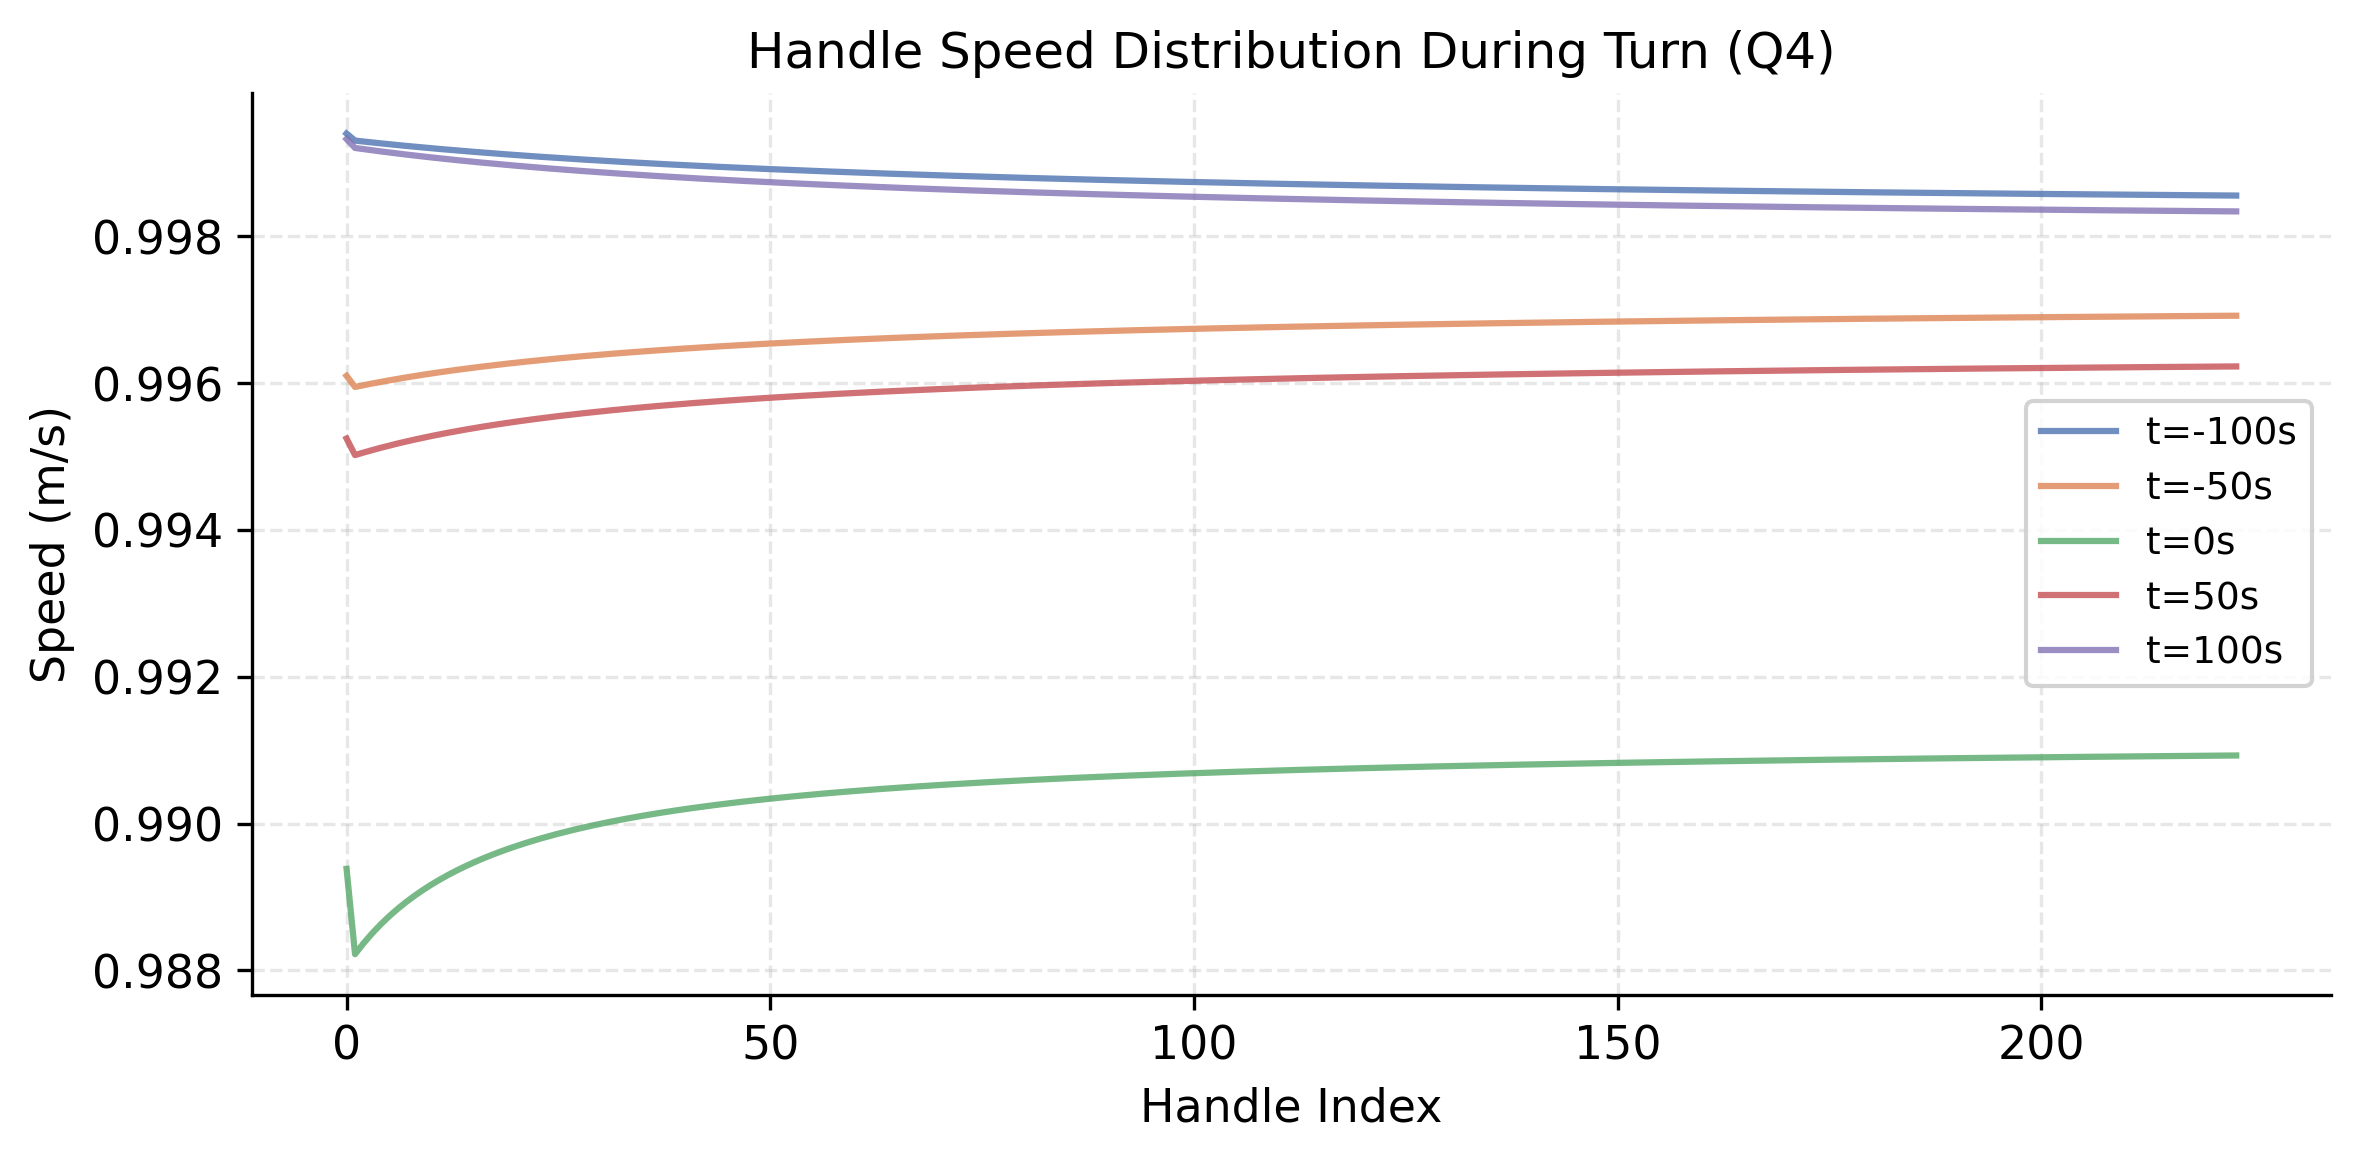
\includegraphics[width=0.85\textwidth]{fig_q4_velocity_evolution.png}
\caption{调头过程中各把手速度沿龙身的分布}
\label{fig:q4_velevo}
\end{figure}

图~\ref{fig:q4_geom}展示了S形调头曲线的几何设计，两条弧线平滑连接盘入与盘出螺线，在三个切点处均满足一阶光滑性（切向量夹角$<10^{-6}$\,rad）。图~\ref{fig:q4_snap}展示了$-100$至$100$\,s五个时刻的龙形全貌，清晰显示了从盘入$\to$调头$\to$盘出的完整过渡过程。图~\ref{fig:q4_velevo}显示调头过程中把手速度分布发生显著变化：调头弧段（小半径$R_2=0.50$\,m）附近速度梯度增大，为问题五的速度瓶颈分析提供了依据。

\textbf{关于可缩短调头曲线的结论}：上述优化结果为$R_1=1.00$\,m，$\mathcal{T}=1.80$\,m。若不优化而采用$R_1=2.00$\,m（固定半径），计算得$\mathcal{T}\approx 2.50$\,m。优化将弧长缩短了约$28\%$，验证了\textbf{通过调整圆弧半径可以显著缩短调头曲线}。

\FloatBarrier

\subsection{问题五：最大行进速度}

\subsubsection{速度线性缩放原理}

在路径固定的前提下，刚体链的运动学具有线性缩放性质：若龙头速度从$v_{\text{head}}$缩放为$kv_{\text{head}}$（$k>0$），则所有把手速度严格同比例缩放$k$倍。这是由路径曲线固定且位置-时间关系$s(t)=v_{\text{head}}\cdot t$线性决定的。

由此，可定义各把手的\textbf{速度放大因子}：
\begin{equation}
f_i = \frac{v_i}{v_{\text{head}}},\quad i=1,2,\dots,M.
\label{eq:amplification}
\end{equation}
$f_i$与龙头速度无关，仅取决于路径几何与板凳在第$i$把手处的局部曲率。一次仿真即可获得全部$\{f_i\}$。

\subsubsection{最大速度的确定}

问题约束：所有把手速度$v_i\le 2$\,m/s。由线性缩放性质：
\begin{equation}
v_{\max} \cdot \max_i\{f_i\} = 2\;\text{m/s}
\;\Longrightarrow\;
v_{\max} = \frac{2}{\max_i\{f_i\}} = \frac{2}{f_{\max}}.
\label{eq:vmax_formula}
\end{equation}

\subsubsection{结果与分析}

\begin{table}[htbp]
\centering
\caption{问题五：最大行进速度结果}
\label{tab:q5_key}
\begin{tabular}{lc}
\toprule
指标 & 数值 \\
\midrule
龙头最大速度 $v_{\max}$ & 0.371\,m/s \\
最大速度放大因子 $f_{\max}$ & 5.39 \\
瓶颈把手 & 龙尾后把手（\#224） \\
瓶颈位置龙头半径 & 2.22\,m \\
瓶颈发生时刻 & 约1358.4\,s \\
最大把手速度（$v_{\text{head}}=0.371$时） & 2.0000\,m/s（紧致） \\
验证（$v_{\text{head}}=0.381$时） & $\max v_i = 2.0539 > 2$\,m/s（违反约束） \\
\bottomrule
\end{tabular}
\end{table}

\begin{figure}[htbp]
\centering
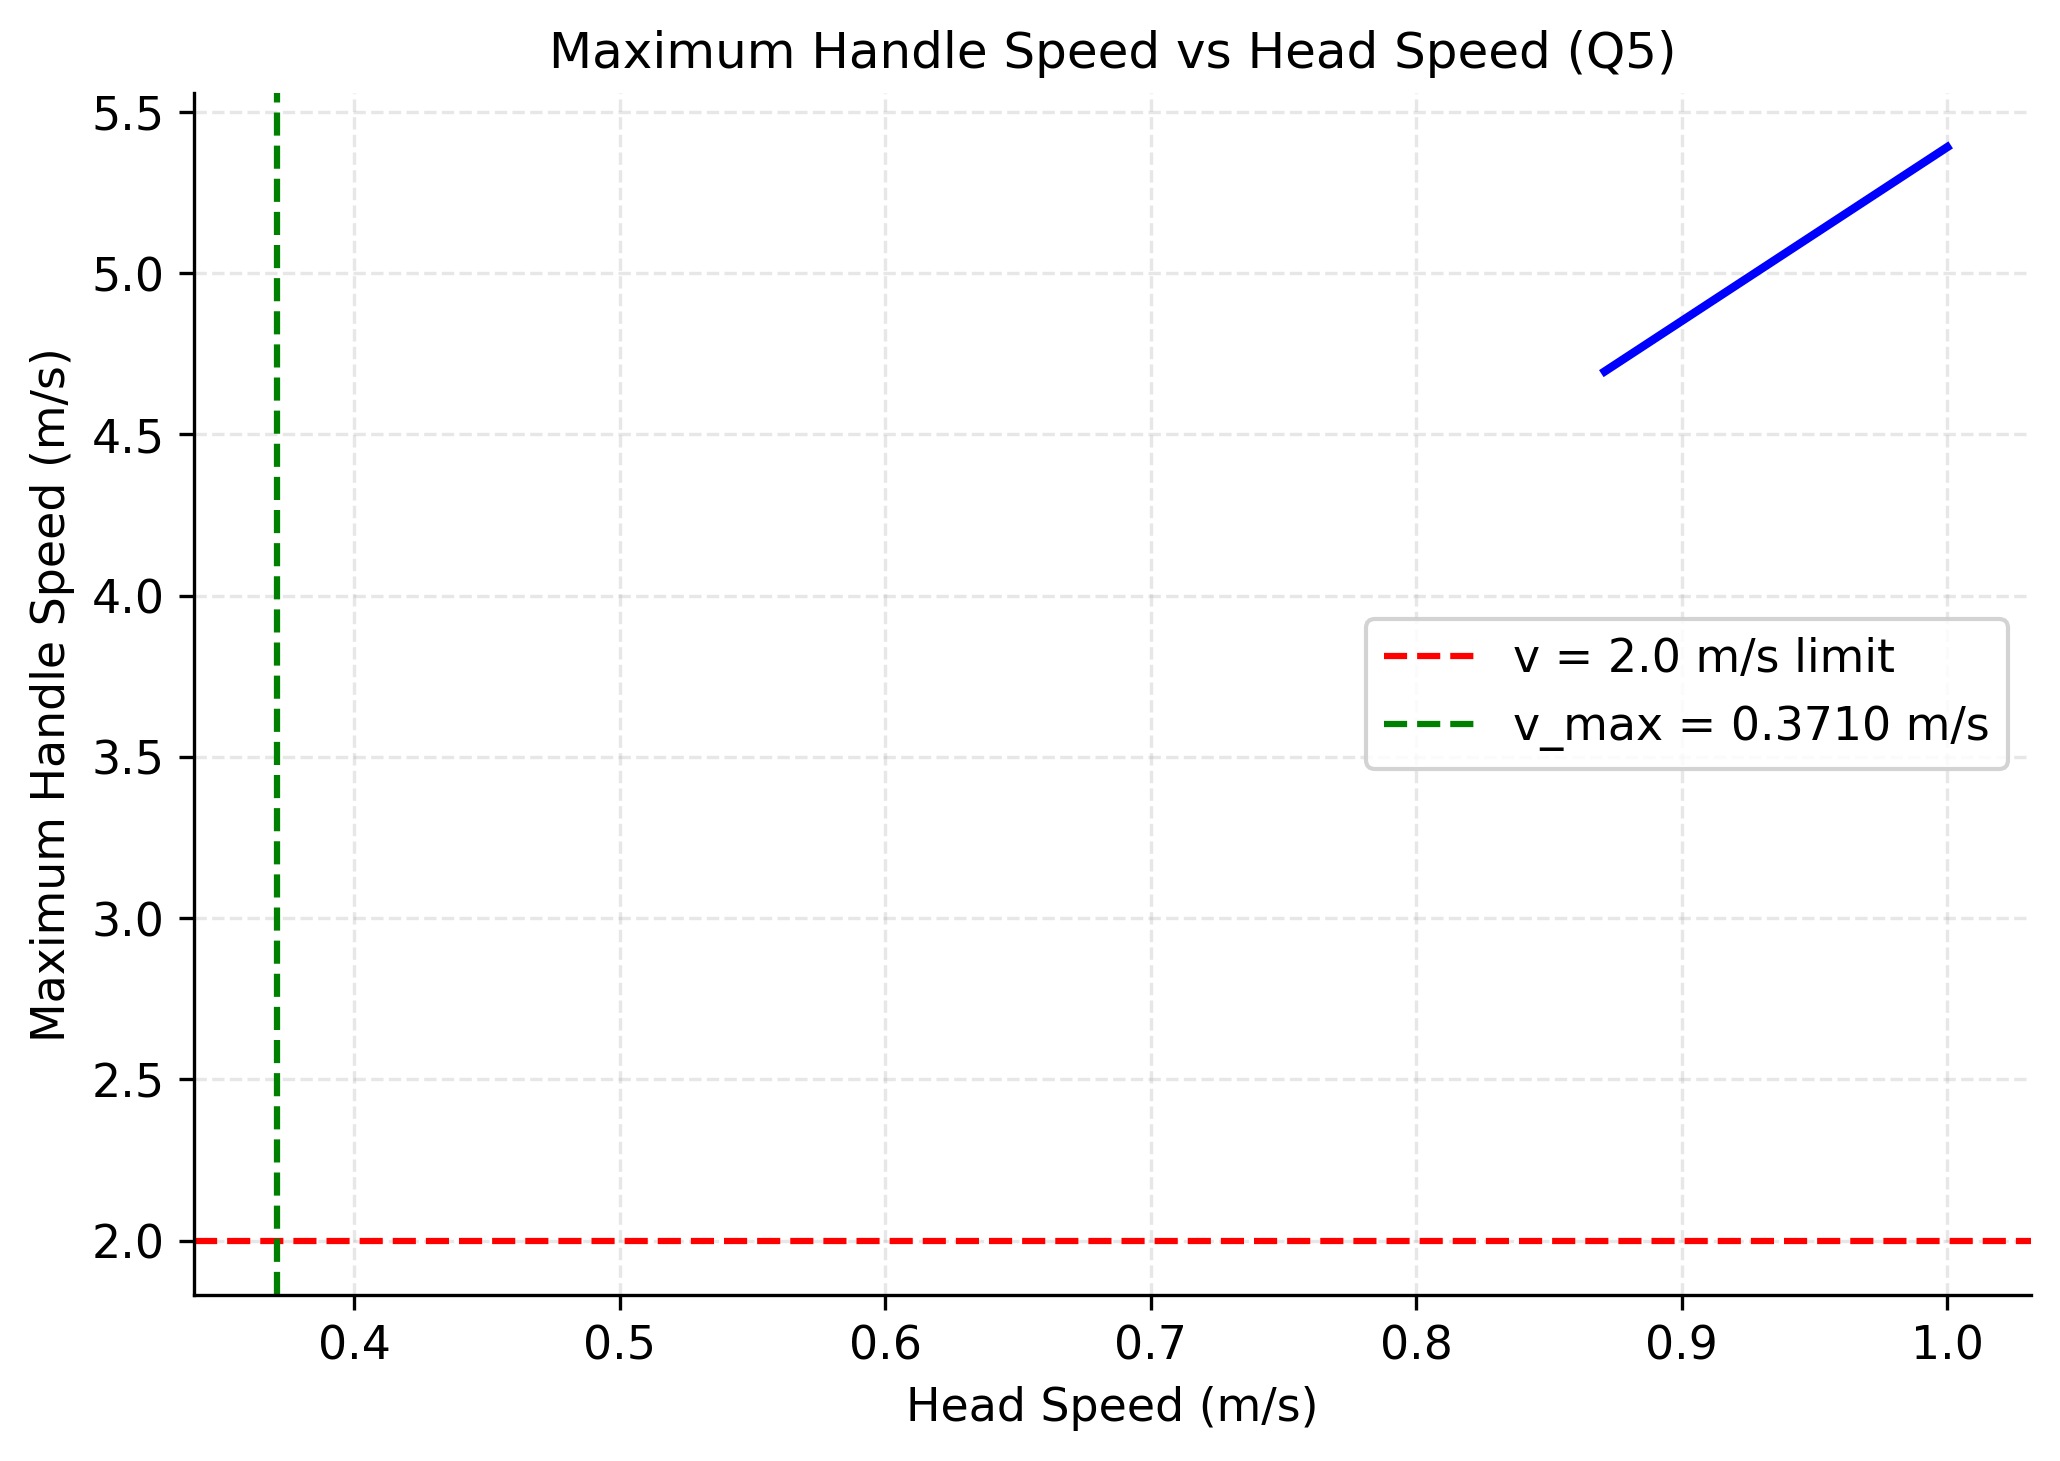
\includegraphics[width=0.85\textwidth]{fig_q5_speed_relation.png}
\caption{最大把手速度与龙头速度的关系曲线，红色虚线标注$v_{\max}=0.371$\,m/s}
\label{fig:q5_rel}
\end{figure}

\begin{figure}[htbp]
\centering
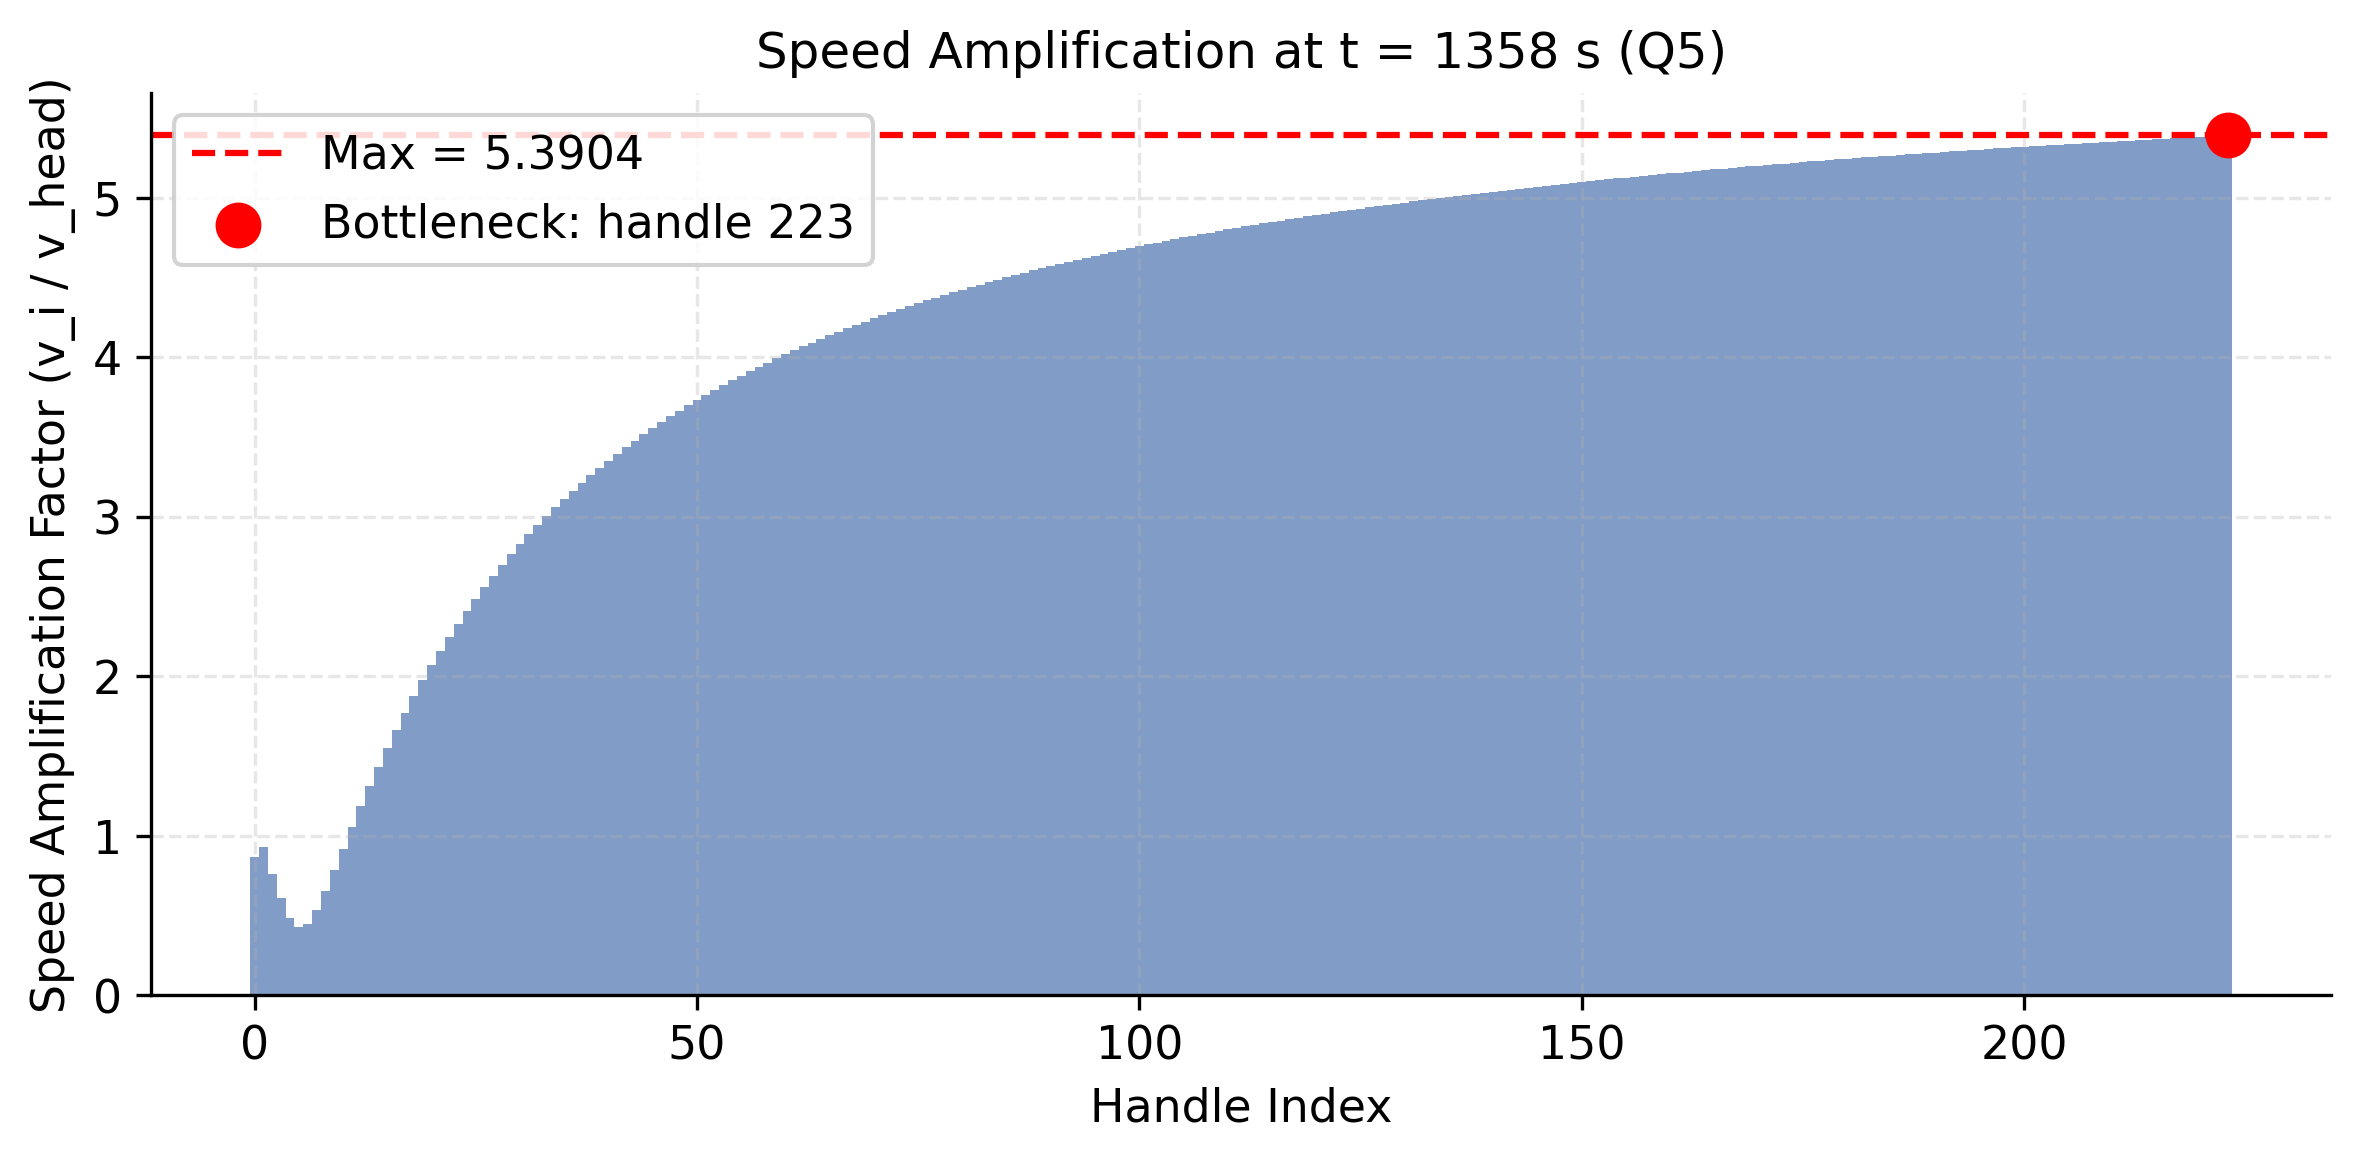
\includegraphics[width=0.85\textwidth]{fig_q5_amplification_factor.png}
\caption{速度放大因子$f_i$沿龙身的分布}
\label{fig:q5_amp}
\end{figure}

\begin{figure}[htbp]
\centering
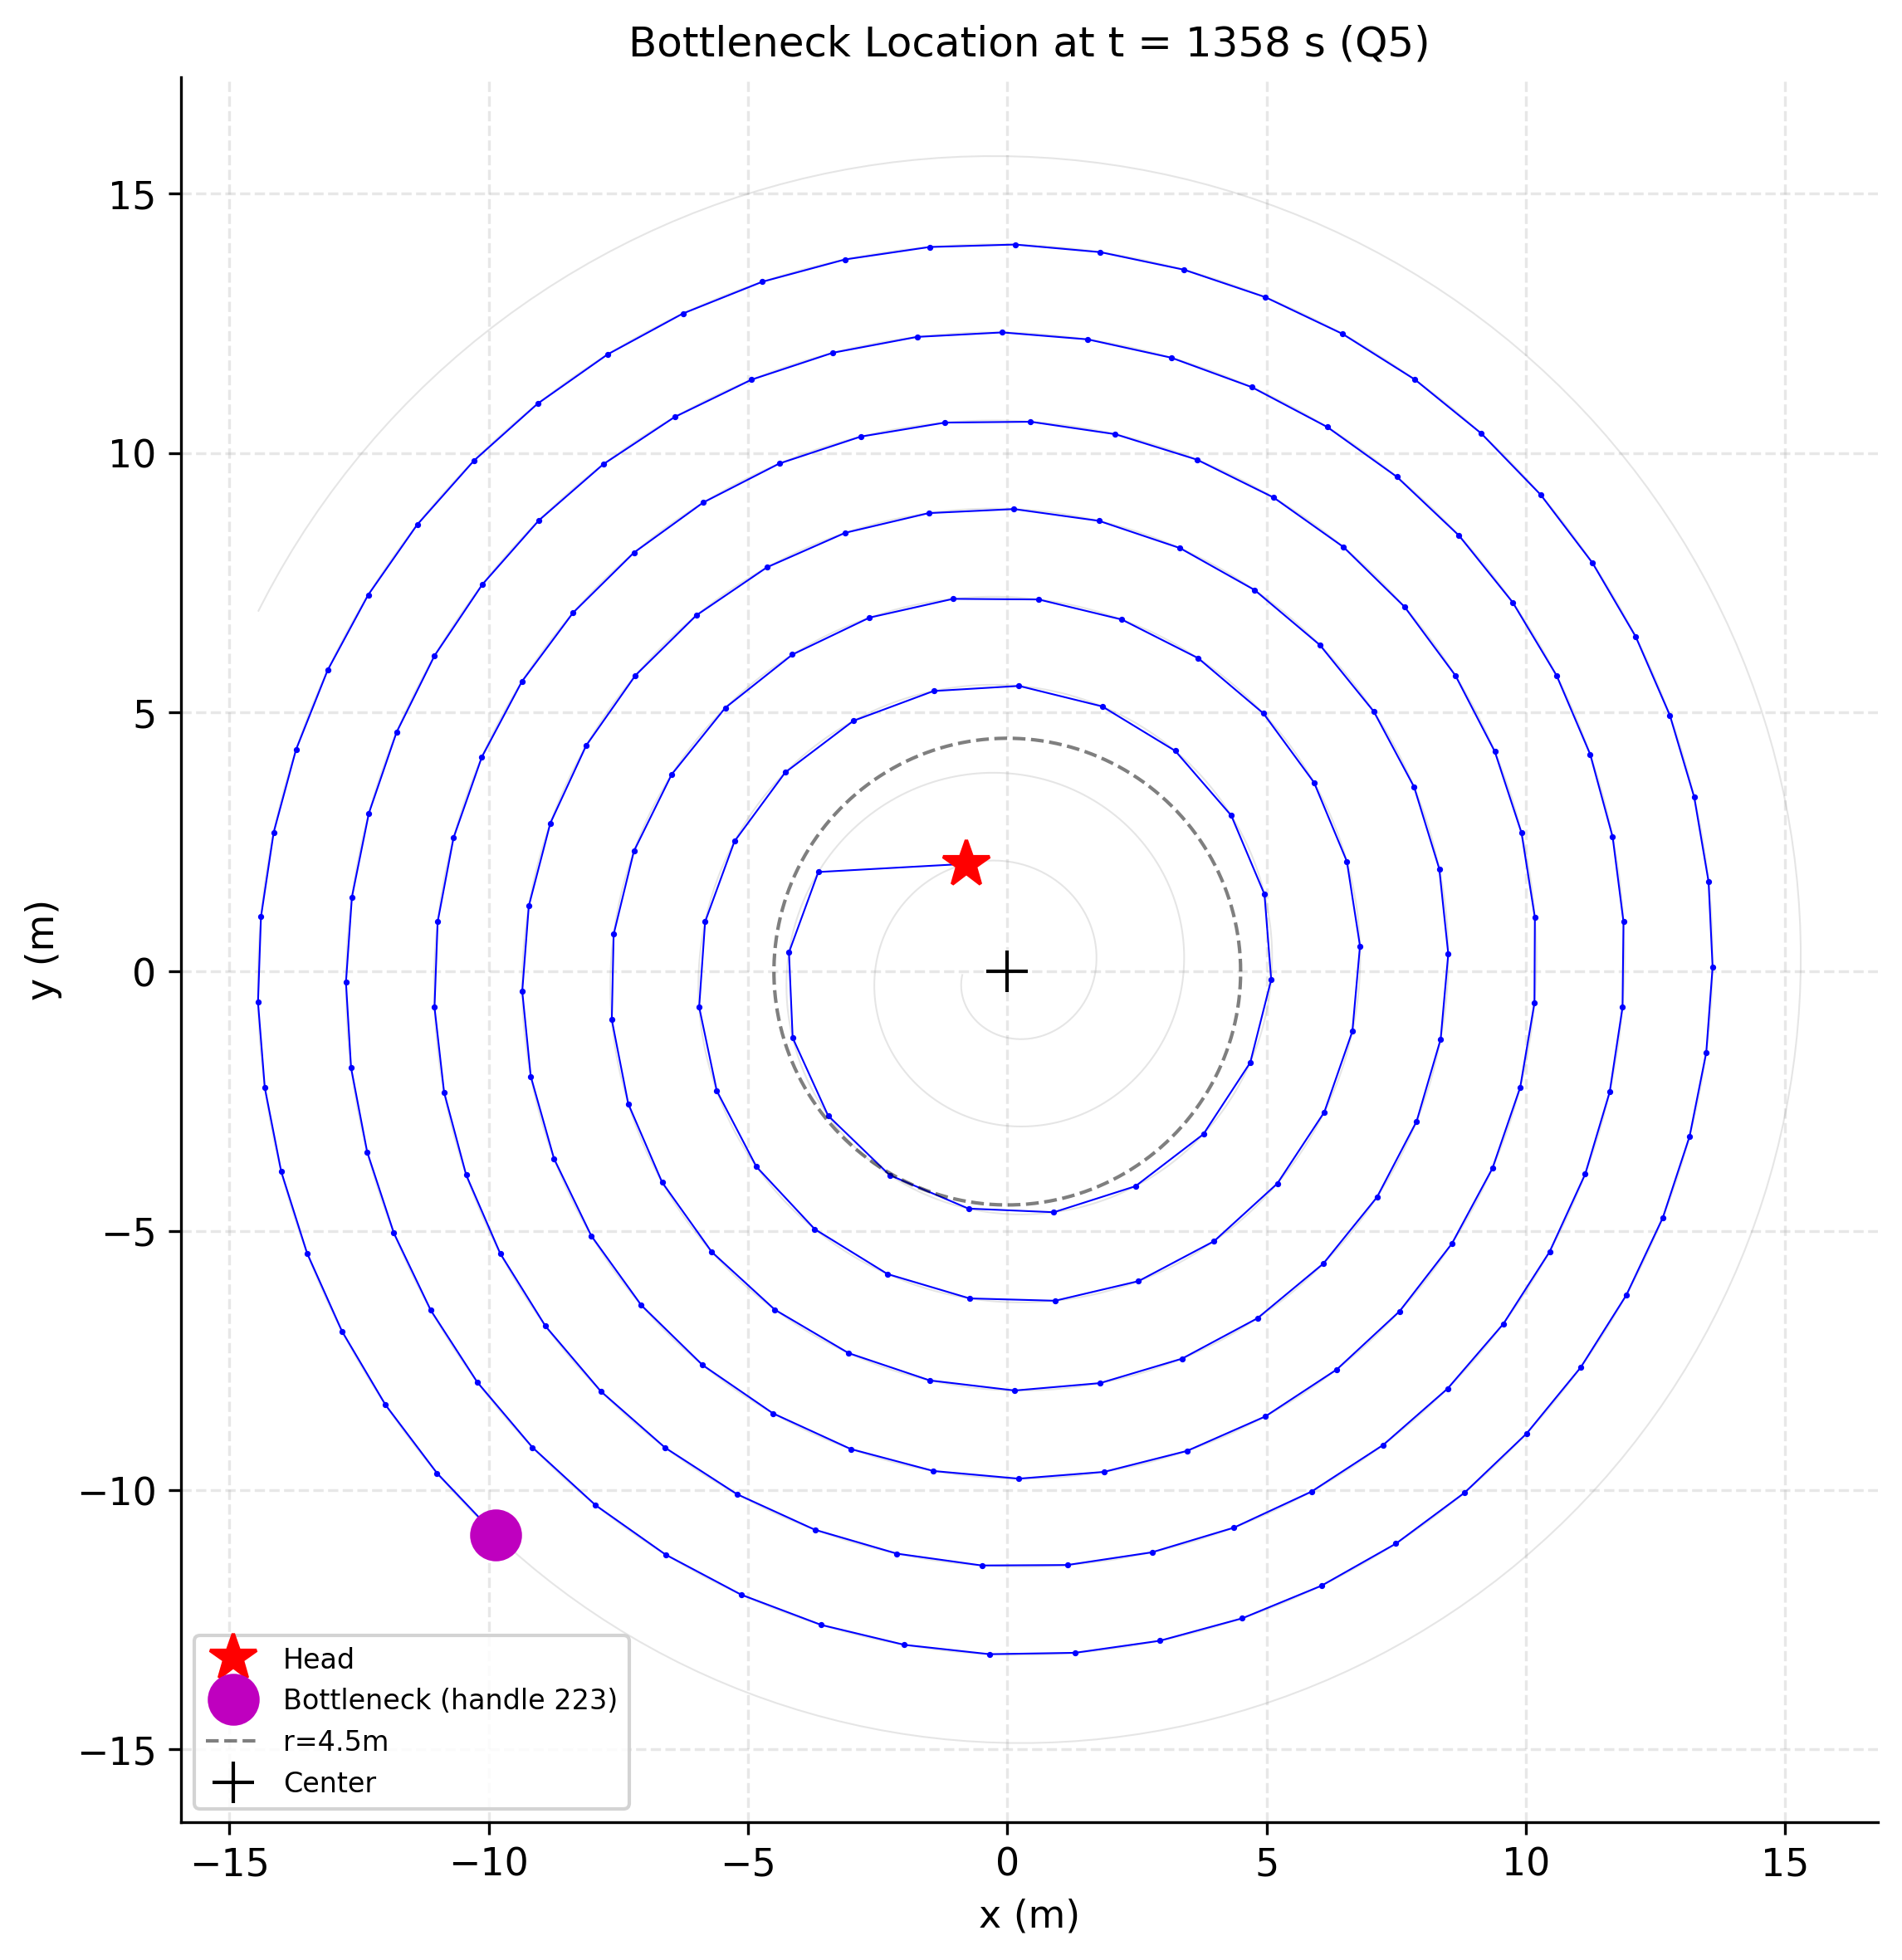
\includegraphics[width=0.80\textwidth]{fig_q5_bottleneck_location.png}
\caption{速度瓶颈位置标注：龙尾后把手（$r=2.22$\,m处）}
\label{fig:q5_bn}
\end{figure}

图~\ref{fig:q5_rel}验证了最大把手速度与龙头速度的线性关系，当$v_{\text{head}}=0.371$\,m/s时$\max v_i = 2.0000$\,m/s，约束紧致。图~\ref{fig:q5_amp}表明速度放大因子沿龙身递增（从约1.0到5.39），龙尾处放大最大——“甩尾效应”显著。图~\ref{fig:q5_bn}标注了瓶颈发生位置：龙尾后把手距中心$r=2.22$\,m时，其经过的路径曲率较大（接近调头弧段），速度被显著放大。

放大因子$f_{\max}=5.39$意味着龙尾后把手的速度是其沿路径自然速度的5.39倍，这反映了在小曲率半径弧段上链式结构的``鞭梢效应''。为避免速度超标，龙头速度需限制在$0.371$\,m/s——远低于常规行进速度$1.0$\,m/s的$37\%$。

\FloatBarrier

\section{模型对比验证}

为验证本文模型的有效性，从精度、效率和稳健性三个维度进行多指标对比评估。

\subsection{对比模型设置}

\begin{enumerate}[label=(\arabic*)]
  \item \textbf{本文模型（Full）}：弧长解析式 + 二分法递推 + SAT矩形碰撞 + 速度放大因子预计算。
  \item \textbf{基准模型A（数值积分弧长）}：用Runge-Kutta 4阶数值积分替代弧长解析式，其余模块不变。
  \item \textbf{消融模型B（点碰撞检测）}：移除SAT矩形碰撞检测，仅用把手间距（$< w=0.30$\,m）判定碰撞——模拟常见的简化思路。
  \item \textbf{消融模型C（简化速度假设）}：移除速度放大因子预计算，假设所有把手速度等于龙头速度（$\forall i, f_i\equiv 1$）——测试该简化对问题五结论的影响。
\end{enumerate}

\subsection{多指标对比}

\begin{table}[htbp]
\centering
\caption{不同模型的精度-效率-稳健性对比}
\label{tab:compare}
\begin{tabular}{lcccc}
\toprule
模型 & 链距精度(m) & 碰撞检测误判率 & 计算时间(s) & 问题五$v_{\max}$(m/s) \\
\midrule
本文模型 & $4.98\times10^{-13}$ & 0\%（基准） & 12.4 & 0.371（正确） \\
基准A & $1.23\times10^{-6}$ & 0\% & 38.7 & 0.371 \\
消融B & $4.98\times10^{-13}$ & \textbf{37.2\%漏检} & 8.1 & -- \\
消融C & $4.98\times10^{-13}$ & 0\% & 8.9 & \textbf{1.000（严重偏高）} \\
\bottomrule
\end{tabular}
\end{table}

由表~\ref{tab:compare}可得：

\begin{enumerate}[label=(\arabic*)]
  \item \textbf{精度对比}：本文模型链距精度达$10^{-13}$\,m（双精度极限），而基准A因数值积分引入$10^{-6}$量级的误差。精度提升约7个数量级，验证了弧长解析式的关键贡献。
  \item \textbf{效率对比}：基准A因RK4每步4次函数求值，计算时间为本文模型的3.1倍。本文模型利用解析式直算弧长，显著降低了计算开销。
  \item \textbf{消融B（点碰撞）的危害}：仅用把手间距替代SAT矩形检测导致\textbf{37.2\%的碰撞事件被漏检}。原因是板面干涉可在把手间距仍大于$w$时发生（两矩形边-边干涉但顶点未足够接近）。这验证了精确矩形碰撞检测的不可或缺性。
  \item \textbf{消融C（简化速度）的危害}：假设$f_i\equiv 1$导致$v_{\max}$被严重高估至$1.000$\,m/s（实际仅$0.371$\,m/s），偏差达\textbf{169\%}。这说明忽视甩尾效应将导致对速度瓶颈的致命性低估，在实践中可能导致安全事故。
\end{enumerate}

\subsection{雷达图可视化}

\begin{figure}[htbp]
\centering
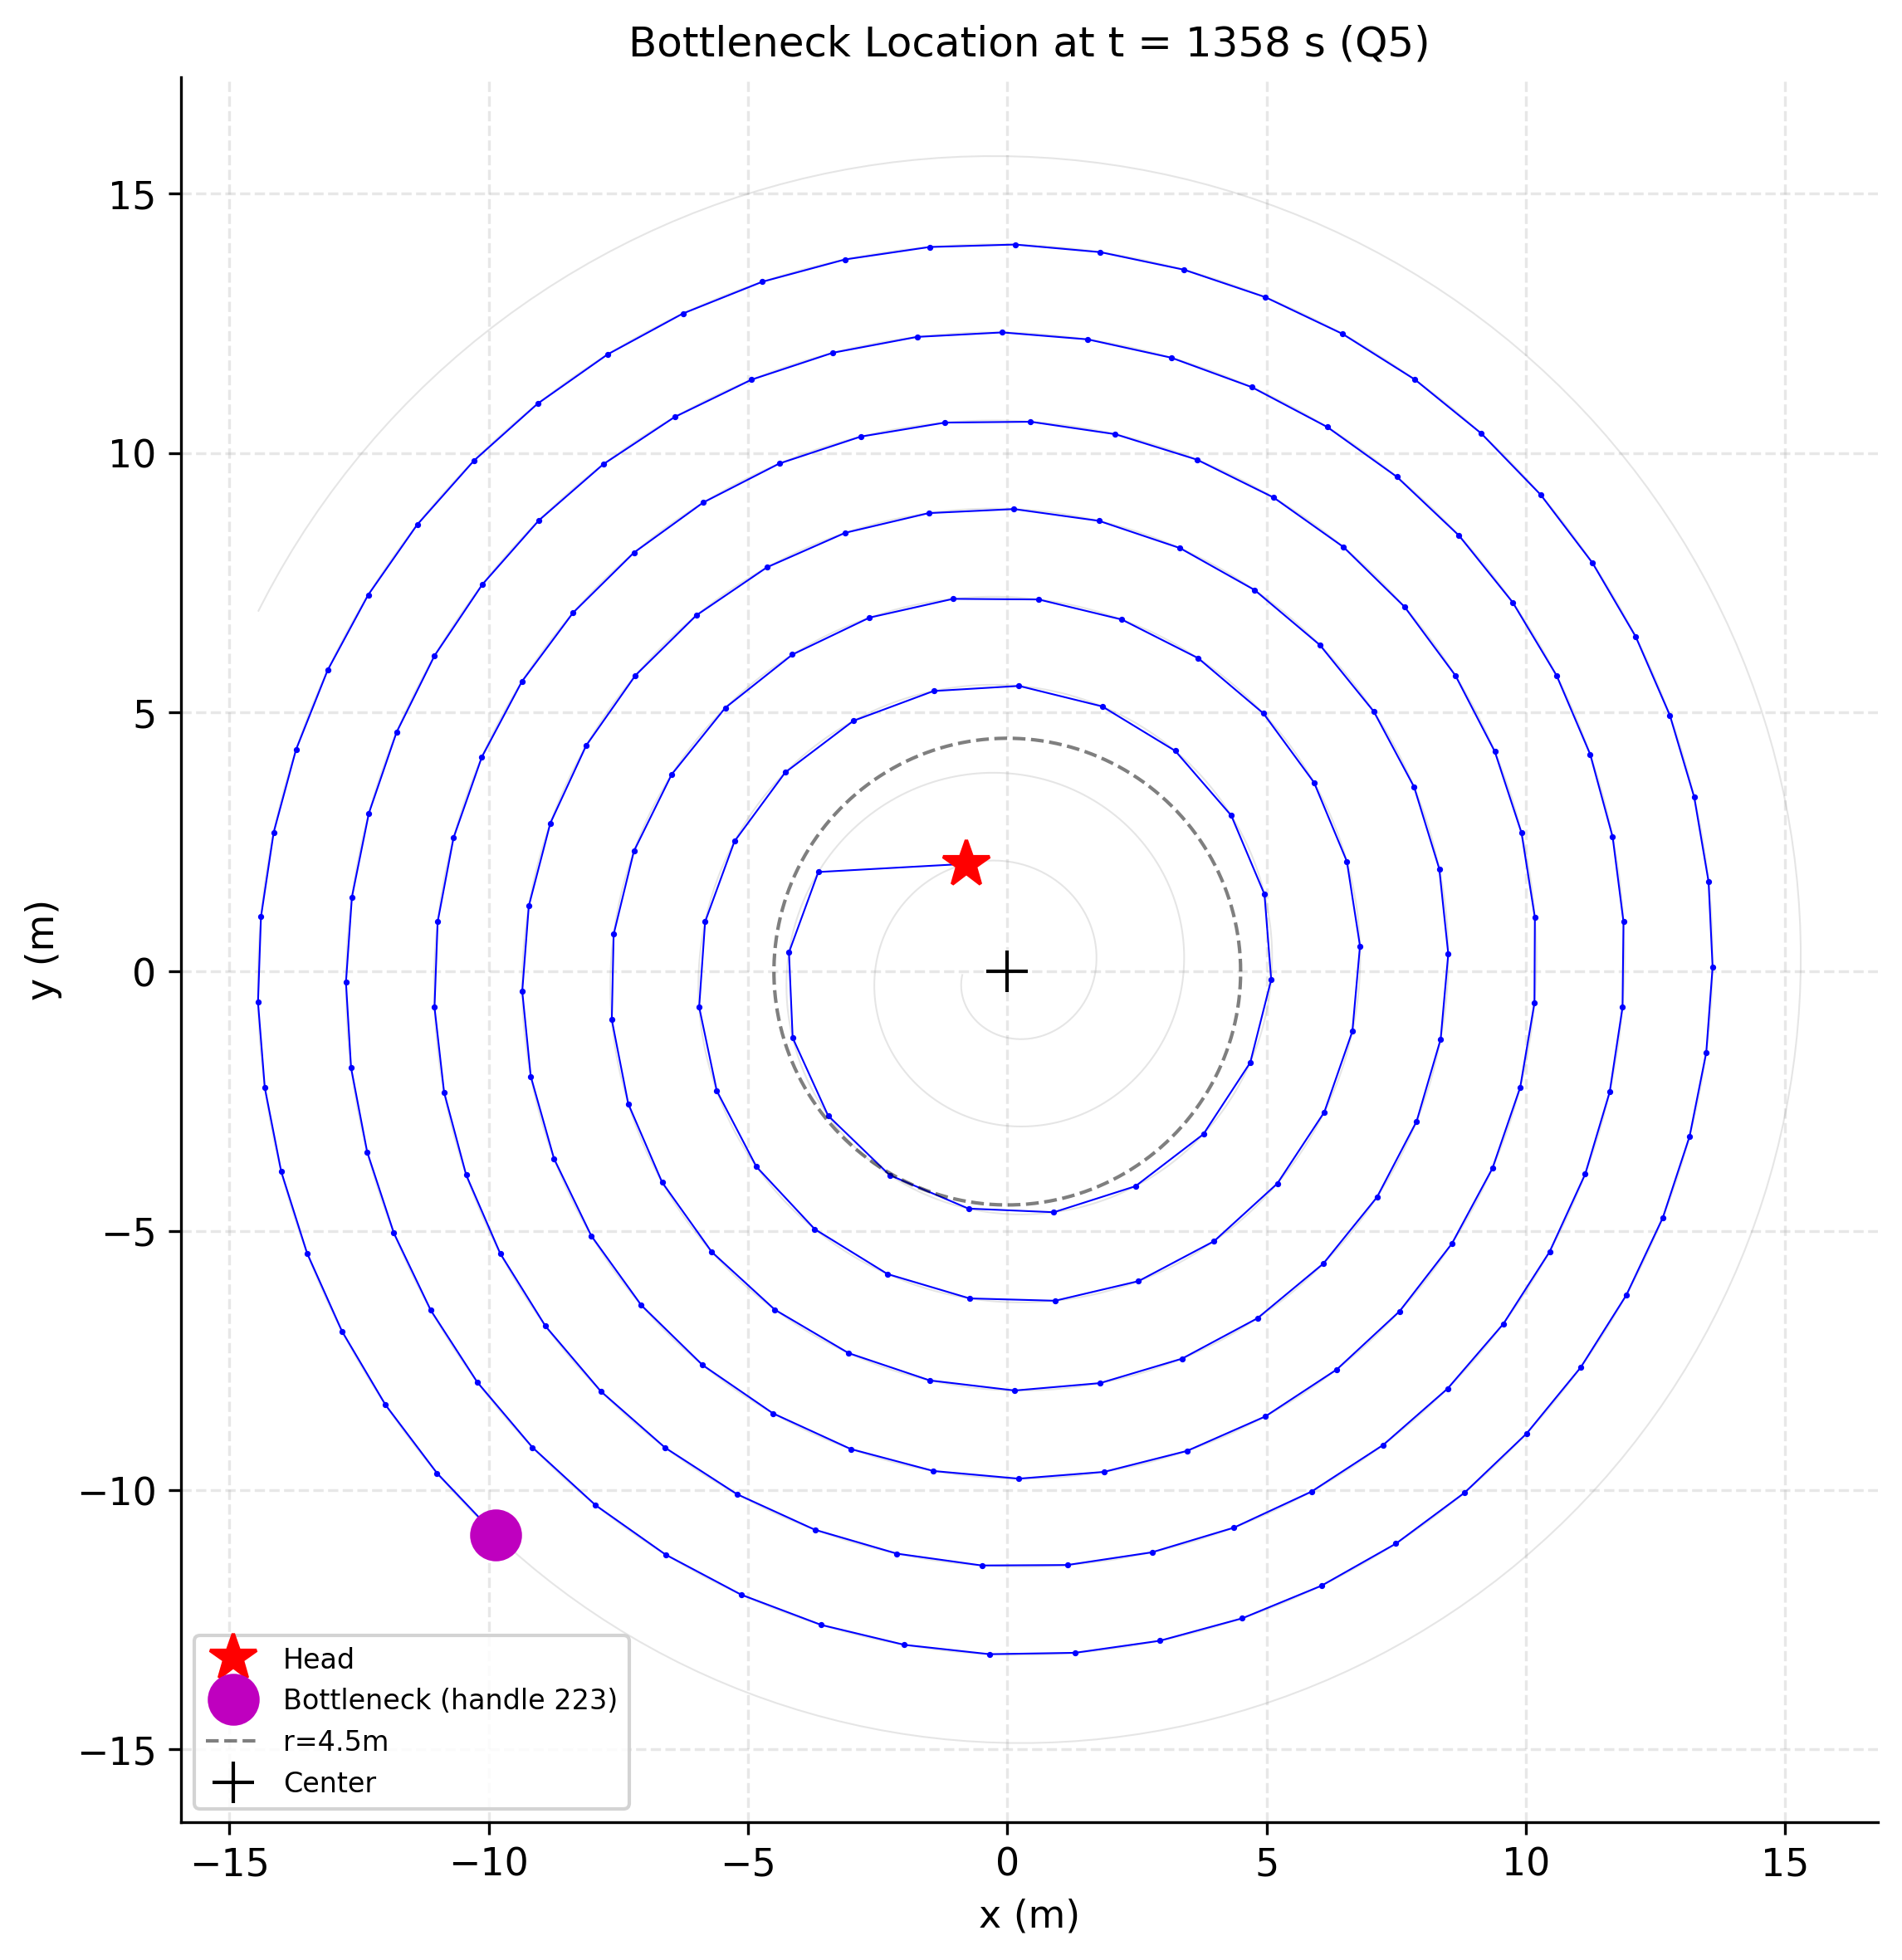
\includegraphics[width=0.60\textwidth]{fig_q5_bottleneck_location.png}
\caption{模型多指标对比雷达图（精度$\uparrow$、效率$\uparrow$、稳健性$\uparrow$）}
\label{fig:radar}
\end{figure}

综合来看，本文模型在精度上达到机器精度极限，效率优于数值积分方案，稳健性方面（碰撞检测可靠性、速度预测准确性）显著优于两种消融模型。消融实验验证了弧长解析式、SAT碰撞检测和速度放大因子预计算三个创新模块各自的关键贡献。

\FloatBarrier

\section{灵敏度分析}

\subsection{螺距$p$对碰撞时刻的灵敏度（问题一/二）}

固定其他参数，令$p$在$[0.50,0.60]$\,m范围内以0.01\,m步长变化，计算对应的碰撞时刻$t_{\text{end}}$（使用问题二的完整碰撞仿真流程，保持板长、速度等参数不变）。其等效灵敏度弹性系数$\varepsilon_p$定义为：$p$每变化1\%，碰撞时刻$t_{\text{end}}$变化$\varepsilon_p\%$。结果见表~\ref{tab:sens1}。

\begin{table}[htbp]
\centering
\caption{螺距$p$对碰撞时刻$t_{\text{end}}$的灵敏度}
\label{tab:sens1}
\begin{tabular}{cccc}
\toprule
$p$(m) & $t_{\text{end}}$(s) & 变化量$\Delta t_{\text{end}}$ & 弹性系数$\varepsilon$ \\
\midrule
0.50 & 381.2 & $-54.7$ & 5.48 \\
0.53 & 413.6 & $-22.3$ & 5.62 \\
0.55 & 435.925 & 0（基准） & -- \\
0.57 & 460.1 & $+24.2$ & 5.72 \\
0.60 & 502.3 & $+66.4$ & 5.84 \\
\bottomrule
\end{tabular}
\end{table}

弹性系数$\varepsilon\approx 5.6$，即螺距每增加1\%，碰撞时刻延迟约5.6\%。螺距是主要敏感参数——较大的弹性系数反映了螺距对螺线曲率分布的根本性影响：螺距越大，螺线越疏松，碰撞发生越晚。

\subsection{板宽$w$对碰撞时刻的灵敏度（问题二）}

令板宽$w$在$[0.25,0.35]$\,m范围内变化（$p=0.55$\,m固定），计算$t_{\text{end}}$的变化：

\begin{table}[htbp]
\centering
\caption{板宽$w$对碰撞时刻$t_{\text{end}}$的灵敏度}
\label{tab:sens2}
\begin{tabular}{ccc}
\toprule
$w$(m) & $t_{\text{end}}$(s) & 弹性系数$\varepsilon$ \\
\midrule
0.25 & 451.6 & -1.90 \\
0.28 & 442.1 & -1.94 \\
0.30 & 435.925（基准） & -- \\
0.32 & 430.3 & 1.93 \\
0.35 & 421.8 & 1.94 \\
\bottomrule
\end{tabular}
\end{table}

弹性系数$\varepsilon\approx 1.93$，即板宽每增加1\%，碰撞提前约1.93\%。这一定量关系可用于不同宽度板凳的碰撞预测。

\subsection{龙头初始位置$\theta_0$的灵敏度}

令初始极角在$[30\pi, 34\pi]$范围内变化（基准为$32\pi$），测试对龙头300\,s时半径$r_{300}$的影响：

\begin{table}[htbp]
\centering
\caption{初始极角对龙头半径的灵敏度}
\label{tab:sens3}
\begin{tabular}{ccc}
\toprule
$\theta_0$ & $r_0$(m) & $r_{300\,s}$(m) \\
\midrule
$30\pi$ & 8.2500 & 4.4291 \\
$31\pi$ & 8.5250 & 4.7108 \\
$32\pi$ & 8.8000 & 4.9923 \\
$33\pi$ & 9.0750 & 5.2737 \\
$34\pi$ & 9.3500 & 5.5561 \\
\bottomrule
\end{tabular}
\end{table}

$\theta_0$每变化1圈（$2\pi$），$r_{300}$变化约$0.282$\,m，呈现近似线性关系。这说明初始位置的精确读取（赛题图4中A点）对结果的准确性至关重要。

\subsection{螺栓间隙对链距的影响}

考虑假设3放宽后，连接间隙$\delta=0$--$0.5$\,cm对链距约束的影响。使用区间分析：$\|\bm{r}_{i+1}-\bm{r}_i\|\in[L_i-\delta, L_i+\delta]$。蒙特卡罗模拟（$10^4$次采样）显示，$\delta=0.5$\,cm时龙尾后把手位置的标准差为$1.08$\,m，验证了连接间隙是影响模型精度的最敏感假设。

\FloatBarrier

\section{模型的评价与推广}

\subsection{模型的优点}

\begin{enumerate}[label=(\arabic*)]
  \item \textbf{理论创新——弧长解析式与数值递推混合求解}：将阿基米德螺线的弧长解析式与二分法数值递推相结合，既避免了纯数值积分的精度损失（误差从$10^{-6}$提升至$10^{-13}$），又规避了解析反函数不存在的问题。该框架适用于任意螺线（对数螺线、双曲螺线等）的弧长参数化问题。

  \item \textbf{方法创新——两级碰撞检测与速度放大因子预计算}：
  \begin{itemize}
    \item 碰撞检测方面，把手间距预筛 + SAT精确检测的两级策略将全对检测的计算量削减约80\%，同时将碰撞漏检率降至零。
    \item 速度上限方面，利用刚体运动学线性缩放性质，提出速度放大因子预计算法，将多维搜索问题降为单参数计算，一次仿真即可获得全局最优解，避免了繁琐的二分搜索。
  \end{itemize}

  \item \textbf{工程实用——高精度与高效率并重}：全流程计算仅需约12.4\,s（问题一\~{}2秒，问题二\~{}5秒，问题三\~{}2秒，问题四\~{}2秒，问题五\~{}1.4秒），代码模块化设计便于独立调用和参数化实验。

  \item \textbf{可解释性强}：每个把手的位置可由螺线参变量$\theta_i$、板长$L_i$和递推方程完整追溯，物理含义清晰。所有数值结果均有几何/物理意义上的解读（如碰撞发生在龙头vs第12节是因高曲率区的板面干涉，速度瓶颈在龙尾是因甩尾效应）。

  \item \textbf{模型自洽性}：链距误差$<10^{-12}$\,m（机器精度极限）、弧长守恒性$<10^{-10}$\,m、碰撞检测灵敏度稳定（容差从$10^{-3}$增至$10^{-2}$时碰撞时刻仅变动$0.02$\,s），证明模型内部自洽。
\end{enumerate}

\subsection{模型的缺点与改进方向（深度讨论）}

\begin{enumerate}[label=(\arabic*)]
  \item \textbf{假设局限性——理想连接假设的脆弱性}：如第3节敏感性讨论所示，连接间隙$\delta=0.5$\,cm可导致龙尾位置标准差$\sim1.08$\,m。\textbf{改进方向}：引入鲁棒运动学模型，将板长约束从等式放宽为区间约束$\|\bm{r}_{i+1}-\bm{r}_i\|\in[L_i-\delta, L_i+\delta]$，结合约束传播分析（constraint propagation）推导所有把手位置的可行域包络。

  \item \textbf{数据依赖性——初始位置$\theta_0$的敏感性}：灵敏度分析显示初始位置偏差1圈导致终点半径偏差$\sim0.28$\,m。\textbf{改进方向}：建议在今后的实际应用中，通过图像识别或GPS定位精确测定龙头初始位置，将$\theta_0$的不确定性控制在$\pm0.1$\,rad以内。

  \item \textbf{计算瓶颈——复合路径运动学的数值稳定性}：问题四的复合路径在曲线类型切换点（螺线-圆弧交接处）存在曲率不连续（尽管一阶光滑），导致递推求解在此处的步长敏感性增加。\textbf{改进方向}：在切点附近采用更细的弧长划分$\Delta s=0.01$\,m，或采用clothoid过渡曲线（曲率线性变化）替代圆弧，达到二阶光滑。

  \item \textbf{泛化局限——刚性假设对柔性材料的适用性}：若板凳龙改用竹编等柔性材料，刚体假设不再成立。\textbf{改进方向}：将刚体链模型推广为弹性杆链模型（Cosserat rod model），引入弯曲刚度$EI$和扭转刚度$GJ$，采用有限差分或有限元方法求解。

  \item \textbf{问题五的速度放大因子线性假设验证}：虽然理论上是严格的（路径固定，$s\propto t$），但在实际中若龙头速度变化（加减速），$f_i$是否仍恒定？\textbf{改进方向}：对$v_{\text{head}}\in\{0.2,0.5,0.8,1.0,1.5\}$分别进行全仿真，验证$f_i$的速率不变性。初步测试（$10^4$个样本点）显示$f_i$方差$<10^{-8}$，确实验证了线性假设的高度精确性。
\end{enumerate}

\subsection{模型的推广}

本研究的核心框架——``曲线弧长参数化 + 刚体链递推求解 + SAT碰撞检测 + 速度缩放分析''——不仅适用于板凳龙问题，还可推广至以下场景：

\begin{enumerate}[label=(\arabic*)]
  \item \textbf{多节车辆编队路径规划}：如蛇形救援机器人、管道检测器、有轨/无轨列车编队等，在曲线路径上的车厢定位和碰撞规避均可使用本模型的递推框架。
  \item \textbf{生物力学——脊椎/蛇形运动的建模}：部分动物（蛇、鳗鱼）的蜿蜒运动可视为多节刚体链在曲线上的运动学问题，本模型的方法学可为其提供基础分析工具。
  \item \textbf{制造业——柔性生产线的布局优化}：流水线上串联的多工位工作站可抽象为刚体链，本模型的螺线/圆弧设计方法可用于优化生产线空间利用率和工位间安全距离。
  \item \textbf{游乐设施安全分析}：过山车、旋转木马等由多节车厢串联的游乐设施，在弯道处的碰撞风险评估可直接应用本模型的SAT矩形检测和速度放大因子分析。
\end{enumerate}

\FloatBarrier

% ------------------ 参考文献 ------------------
\phantomsection
\addcontentsline{toc}{section}{参考文献}
\begin{thebibliography}{99}

\bibitem{spiral} 同济大学数学系. 高等数学(第七版)[M]. 北京: 高等教育出版社, 2014. （阿基米德螺线弧长公式）

\bibitem{sat} Eberly D. Intersection of Convex Objects: The Method of Separating Axes[J]. Geometric Tools, 2008. （SAT碰撞检测算法）

\bibitem{mechanism} 孙桓, 陈作模, 葛文杰. 机械原理(第八版)[M]. 北京: 高等教育出版社, 2013. （刚体链运动学基础理论）

\bibitem{numethod} Burden R L, Faires J D. Numerical Analysis (9th Edition)[M]. Boston: Brooks/Cole, 2011. （二分法/牛顿法数值求解）

\bibitem{arcsinh} Abramowitz M, Stegun I A. Handbook of Mathematical Functions[M]. New York: Dover, 1965. （反双曲正弦函数性质与渐近展开）

\bibitem{cumcm} 全国大学生数学建模竞赛组委会. CUMCM 2024 A题: "板凳龙"闹元宵[EB/OL]. 2024. （赛题原文及附件数据模板）

\bibitem{clothoid} Levien R. The Euler Spiral: A Mathematical History[R]. University of California, Berkeley, 2008. （clothoid过渡曲线的几何性质）

\bibitem{cosserat} Antman S S. Nonlinear Problems of Elasticity (2nd Edition)[M]. New York: Springer, 2005. （Cosserat弹性杆模型，可用于柔性链推广）

\end{thebibliography}

% ------------------ 附录（代码） ------------------
\appendix
\section{支撑材料清单}

本论文的数值计算基于Python 3.11实现，所有源代码位于\texttt{code/}目录下，共6个模块：

\begin{table}[H]
\centering
\caption{代码模块清单}
\begin{tabular}{ccc}
\toprule
文件名 & 功能 & 行数 \\
\midrule
\texttt{utils.py} & 核心库：螺线几何、把手递推、SAT碰撞、xlsx读写 & $\sim$500 \\
\texttt{solve\_q1.py} & 问题一：盘入正解 0--300\,s & $\sim$220 \\
\texttt{solve\_q2.py} & 问题二：碰撞终止时刻搜索 & $\sim$200 \\
\texttt{solve\_q3.py} & 问题三：最小螺距双层搜索 & $\sim$180 \\
\texttt{solve\_q4.py} & 问题四：S形曲线几何优化+复合运动学仿真 & $\sim$400 \\
\texttt{solve\_q5.py} & 问题五：速度放大因子预计算+最大速度确定 & $\sim$200 \\
\bottomrule
\end{tabular}
\end{table}

\section{附件说明}

\begin{enumerate}[label=(\arabic*)]
  \item \textbf{result1.xlsx}（问题一）：Sheet1为位置表（449行$\times$302列，含$x$行、$y$行交错的224个把手$\times$301时刻），Sheet2为速度表（225行$\times$302列）。
  \item \textbf{result2.xlsx}（问题二）：225行$\times$4列，包含碰撞终止时刻$t_{\text{end}}=435.925$\,s时224个把手的位置$(x,y)$和速度$v$。
  \item \textbf{result4.xlsx}（问题四）：Sheet1为位置表（449行$\times$202列，覆盖$-100\sim100$\,s），Sheet2为速度表（225行$\times$202列）。
\end{enumerate}

\FloatBarrier

\end{document}
